% !Mode:: "TeX:DE:UTF-8:Main"
%
%
%JOURNAL CODE  SEE DOCUMENTATION

\documentclass[MAL,biber]{nowfnt} % creates the journal version, needs biber version
%wrapper for book and ebook are created automatically.

\usepackage[utf8]{inputenc}
\usepackage{amsmath,amssymb,amsthm}
\usepackage{graphicx, graphics, epsfig, color}
\usepackage{tikz, pgfplots}
\usetikzlibrary{plotmarks,decorations.pathreplacing}
\pgfplotsset{compat=newest}
\usepackage{hyperref}
\hypersetup{colorlinks=false}
%\usepackage{subfigure}
\usepackage{subcaption}

% define color
\definecolor{RED}{rgb}{0.7,0,0}
\definecolor{BLUE}{rgb}{0,0,0.69}
\definecolor{GREEN}{rgb}{0,0.6,0}
\definecolor{PURPLE}{rgb}{0.69,0,0.8}

%text color
\newcommand{\RED}{\color[rgb]{0.70,0,0}}
\newcommand{\BLUE}{\color[rgb]{0,0,0.69}}
\newcommand{\GREEN}{\color[rgb]{0,0.6,0}}
\newcommand{\PURPLE}{\color[rgb]{0.69,0,0.8}}

\newtheorem{Assumption}{Assumption}
\newtheorem{Theorem}{Theorem}
\newtheorem{Corollary}{Corollary}
\newtheorem{Proposition}{Proposition}
\newtheorem{Lemma}{Lemma}
\newtheorem{Remark}{Remark}
\newtheorem{Definition}{Definition}

% a few definitions that are *not* needed in general:
\newcommand{\ie}{\emph{i.e.}}
\newcommand{\eg}{\emph{e.g.}}
\newcommand{\etc}{\emph{etc}}
\newcommand{\now}{\textsc{now}}

%%% math operators
\newcommand{\T}{{\sf T}}
\DeclareMathOperator{\tr}{tr}
\DeclareMathOperator{\diag}{diag}
\DeclareMathOperator{\rank}{rank}
\DeclareMathOperator{\Cov}{Cov}
\renewcommand{\vec}{{\rm vec}}

\newcommand{\cd}{{ \xrightarrow{d} }}
\newcommand{\asto}{{ \xrightarrow{a.s.} }}

%%% shortcuts
\newcommand{\A}{{\mathbf{A}}}
\newcommand{\B}{{\mathbf{B}}}
\newcommand{\C}{{\mathbf{C}}}
\newcommand{\D}{{\mathbf{D}}}
\newcommand{\E}{{\mathbf{E}}}

\newcommand{\I}{{\mathbf{I}}}
\newcommand{\J}{{\mathbf{J}}}
\newcommand{\K}{{\mathbf{K}}}
\newcommand{\M}{{\mathbf{M}}}
\renewcommand{\P}{{\mathbf{P}}}
\newcommand{\Q}{{\mathbf{Q}}}
\renewcommand{\S}{{\mathbf{S}}}
\newcommand{\U}{{\mathbf{U}}}
\newcommand{\V}{{\mathbf{V}}}
\newcommand{\W}{{\mathbf{W}}}
\newcommand{\X}{{\mathbf{X}}}
\newcommand{\Y}{{\mathbf{Y}}}
\newcommand{\Z}{{\mathbf{Z}}}

\renewcommand{\a}{{\mathbf{a}}}
\renewcommand{\b}{{\mathbf{b}}}
\renewcommand{\j}{{\mathbf{j}}}
\renewcommand{\t}{{\mathbf{t}}}
\newcommand{\uu}{{\mathbf{u}}}
\renewcommand{\v}{{\mathbf{v}}}
\newcommand{\x}{{\mathbf{x}}}
\newcommand{\y}{{\mathbf{y}}}
\newcommand{\z}{{\mathbf{z}}}



\newcommand{\bmu}{{ \boldsymbol{\mu} }}
\newcommand{\bLambda}{{ \boldsymbol{\Lambda} }}

\newcommand{\zo}{{\mathbf{0}}}
\newcommand{\one}{{\mathbf{1}}}

\newcommand{\RR}{{\mathbb{R}}}
\newcommand{\CC}{{\mathbb{C}}}
\newcommand{\EE}{{\mathbb{E}}}
\newcommand{\NN}{{\mathcal{N}}}

%ARTICLE TITLE
\title{Random Matrix Advances in Modern Machine Learning}


%ARTICLE SUB-TITLE
%\subtitle{Instructions for Creating an FnT Article}


%AUTHORS FOR COVER PAGE 
% separate authors by \and, item by \\
% Don't use verbatim or problematic symbols.
% _ in mail address should be entered as \_
% Pay attention to large mail-addresses ...

%if there are many author twocolumn mode can be activated.
%\booltrue{authortwocolumn} %SEE DOCUMENTATION
\maintitleauthorlist{
Alet Heezemans \\
now publishers, Inc. \\
alet.heezemans@nowpublishers.com
\and
Mike Casey \\
now publishers, Inc. \\
mike.casey@nowpublishers.com
}

%ISSUE DATA AS PROVIDED BY NOW
\issuesetup
{%
 copyrightowner={A.~Heezemans and M.~Casey},
 volume        = xx,
 issue         = xx,
 pubyear       = 2018,
 isbn          = xxx-x-xxxxx-xxx-x,
 eisbn         = xxx-x-xxxxx-xxx-x,
 doi           = 10.1561/XXXXXXXXX,
 firstpage     = 1, %Explain
 lastpage      = 18
 }

%BIBLIOGRAPHY FILE
\addbibresource{liao.bib}

\usepackage{mwe}

%AUTHORS FOR ABSTRACT PAGE
\author[1]{Heezemans,Alet}
\author[2]{Casey,Mike}

\affil[1]{now publishers, Inc.; alet.heezemans@nowpublishers.com}
\affil[2]{now publishers, Inc.; mike.casey@nowpublishers.com}

\articledatabox{\nowfntstandardcitation}

\begin{document}

\makeabstracttitle

\begin{abstract}
to be done

\end{abstract}

\chapter{Introduction}
\label{chap:intro} 

\section{Motivation: the pitfalls of large dimensional statistics}
\label{sec:motivation}

\subsection{The big data era: when $n$ is no longer much larger than $p$}

The big data revolution comes along with the challenge need to parse, mine, compress large amount of large dimensional and possibly heterogeneous data. In many applications, the dimension $p$ of the observations is as large as -- if not much larger than -- their number $n$. In array processing and wireless communications, the number of antennas required for fine localization resolution or increased communication throughput may be as large (today in the order of hundreds) as the number of available independent signal observations \citep{lu2014overview,li2007mimo}. In genomics, the identification of correlations among hundred of thousands genes based on a limited number of independent (and expensive) samples induces an even larger ratio $p/n$ \citep{arnold1994evolutionary}. In statistical finance, portfolio optimization relies on the opposite need to invest on a large number $p$ of assets to reduce volatility but at the same time to estimate the current (rather than past) asset statistics from a relatively small number $n$ of asset return records \citep{laloux2000random}. 

As we shall demonstrate in the next section, the fact that in these problems $n$ is not \emph{much larger} than $p$ annihilates most of the results from standard asymptotic statistics that assume $n$ alone is large \citep{van2000asymptotic}. As a rule of thumb, by \emph{much larger} we mean here that $n$ must be at least $100$ times as large as $p$ for standard asymptotic statistics to be of practical convenience (see our argument in Section~\ref{sec:intro-SCM}). Many algorithms in statistics, signal processing, and machine learning are precisely derived from this inappropriate $n\gg p$ assumption. A main objective of this monograph is to cast a light on the resulting biases and problems incurred and to provide a systematic random matrix framework to improve these algorithms.

Possibly more importantly, we will see along this monograph that finite-dimensional intuitions which are at the core of many machine learning algorithms (starting with spectral clustering \citep{ng2002spectral,von2007tutorial}) may strikingly fail when applied in a simultaneously large $n,p$ setting. A compelling example lies in the notion of ``distance'' between vectors. Most classification methods in machine learning are rooted in the observation that random vectors arising from a mixture distribution (say Gaussian) gather in patches of close-by vectors in Euclidean norm. When dealing with large dimensions, concentration phenomena arise that may make Euclidean distances useless, if not counter-productive: vectors of the same Gaussian mixture class may be further away in Euclidean distance than vectors arising from different classes, but classification may still be doable. The monograph intends to prepare the reader for these multiple traps caused by the famous ``curse of dimensionality''.

\subsection{Sample covariance matrices in the large $n,p$ regime}
\label{sec:intro-SCM}

Let us consider the following illustrating example which shows a first elementary, yet counter-intuitive, result: for simultaneously large $n,p$, sample covariance matrices $\hat\C\in\RR^{p\times p}$ based on $n$ samples $\x_i\sim \NN(\zo,\C)$ are \emph{entry-wise} consistent estimators of the population covariance $\C\in\RR^{p\times p}$ (i.e., $\|\hat\C-\C\|_\infty\to 0$ as $p,n\to \infty$) while overall being extremely poor estimators (i.e., $\|\hat\C-\C\|\not\to 0$ with here $\|\cdot\|$ the operator norm). Matrix norms are in particular \emph{not} equivalent from a large $n,p$ standpoint. 

\medskip

Let us detail this claim, in the simplest case where $\C=\I_p$. Consider a data set $\X = [\x_1, \ldots, \x_n] \in \RR^{p \times n}$ of $n$ independent and identically distributed (i.i.d.\@) observations from a $p$-dimensional Gaussian distribution, i.e., $\x_i \sim \NN(\zo_p, \I_p)$ for $i=1,\ldots,n$. We wish to estimate the population covariance matrix $\C = \I_p$ from the $n$ available samples. The maximum likelihood estimator in this zero-mean Gaussian setting is the sample covariance matrix $\hat \C$ defined by
\begin{equation}\label{eq:scm}
    \hat \C = \frac1n \sum_{i=1}^n \x_i \x_i^\T = \frac1n \X \X^\T.
\end{equation}
By the strong law of large numbers, for fixed $p$, $\hat \C \to \I_p$ almost surely as $n \to \infty$, so that $\| \hat \C - \I_p \| \asto 0$ holds for any standard matrix norm and in particular for the operator norm. 

\medskip

One must be more careful when dealing with the regime $n,p \to \infty$ with ratio $p/n \to c \in (0, \infty)$ (or, from a practical standpoint, $n$ is not much larger than $p$). First, note that the entry-wise convergence still holds since, invoking by the law of large numbers again
\begin{equation*}
    %\hat \C_{i,j} = \frac1n\sum_{l=1}^n \X_{il}\X_{jl} \asto \left\{ \begin{array}{ll} 1, &i=j \\ 0, &i\neq j. \end{array} \right.
    \hat \C_{i,j} = \frac1n\sum_{l=1}^n \X_{i,l}\X_{j,l} \asto \begin{cases} 1, & i=j; \\ 0, &i \neq j. \end{cases}
\end{equation*}
Besides, by a concentration inequality argument, it can even be shown that
\begin{equation*}
    \max_{1\leq i,j\leq p} \left| (\hat \C - \I_p)_{i,j} \right| \asto 0
\end{equation*}
which holds as long as $p$ is no larger than a polynomial function of $n$, and thus
\begin{equation*}
    \|\hat \C-\I_p\|_\infty \asto 0
\end{equation*}
with $\|\A\|_\infty$ the largest absolute entry of matrix $\A$.

Consider now the case $p > n$. Since $\hat \C$ is the sum of $n$ rank one matrices (as per the form \eqref{eq:scm}), the rank of $\hat\C$ is \emph{at most} equal to $n$ and thus, being a $p\times p$ matrix with $p<n$, is a singular matrix having at least $p - n>0$ null eigenvalues. As a consequence, 
\begin{equation*}
    \| \hat \C - \I_p \| \not\to 0
\end{equation*}
for $\|\cdot\|$ the matrix operator (or spectral) norm. This last result actually extends to the general case where $n,p\to\infty$ with $p/n\to c>0$. As such, as claimed above, matrix norms cannot be considered equivalent in the regime where $p$ is not negligible compared to $n$. This follows from the fact that the equivalence factors depend on the matrix size $p$; here for instance, $\|\A\|_\infty\leq \|\A\|\leq p\|\A\|_\infty$ for $\A \in \RR^{p \times p}$.

Unfortunately in practice, as justified by the following remark, the (non converging) operator norm is of more practical interest than the (converging) infinity norm.
\begin{remark}[On the importance of operator norm]\label{rem:operator-norm}
For practical purposes, this loss of norm equivalence raises the question of the relevant matrix norm to be considered in any given application. For the purpose of the present monograph, and for most applications in machine learning, the operator (or spectral) norm is the most relevant. Indeed, first, the operator norm is the matrix norm induced by the Euclidean norm of vectors. Thus, the study of regression vectors or label/score vectors in classification is naturally attached to the spectral study of matrices. Besides, we will often be interested in the asymptotic \emph{equivalence} of families of large dimensional matrices. If $\|\A_p-\B_p\|\to 0$ for matrix sequences $\{\A_p\}$ and $\{\B_p\}$, then according to Weyl's inequality (see for example Theorem~4.3.1 in \citep{horn2012matrix}),
\begin{equation*}
    \max_i \left| \lambda_i(\A_p) -\lambda_i(\B_p) \right| \to 0
\end{equation*}
for $\lambda_1(\A)\geq \lambda_2(\A)\geq \ldots$ the eigenvalues of $\A$ in a decreasing order. Besides, for $\uu_i(\A_p)$ an eigenvector of $\A_p$ associated with an \emph{isolated eigenvalue} $\lambda_i(\A_p)$ (i.e., such that $\min ( |\lambda_{i+1}(\A_p)-\lambda_i(\A_p) |,|\lambda_i(\A_p)-\lambda_{i-1} (\A_p) | )>\varepsilon$ for some $\varepsilon>0$ uniformly on $p$),
\begin{equation*}
    \left\| \uu_i(\A_p) -\uu_i(\B_p) \right\| \to 0.
\end{equation*}
These results ensure that, as far as spectral properties are concerned, $\A_p$ can be studied equivalently through $\B_p$. We will often use this argument to study intractable random matrices $\A_p$ by means of a tractable ersatz $\B_p$.

The pitfall that consists in assuming that $\hat\C$ is a valid estimator of $\C$ since $\|\hat \C-\C\|_\infty \asto 0$ may thus have deleterious practical consequences when $n$ is not significantly larger than $p$.
\end{remark}

Resuming on our norm convergence discussion, it is now natural to ask whether $\hat \C$, which badly estimates $\C$, has a controlled asymptotic behavior. There precisely lay the first theoretical interests of random matrix theory. While $\hat\C$ itself does not converge in any useful way, its eigenvalue distribution does exhibit a traceable limiting behavior \citep{marvcenko1967distribution,silverstein1995empirical,bai2010spectral}. The seminal result in this direction, due to Mar\u{c}enko and Pastur states that, in the case of $\C = \I_p$, as $n,p \to \infty $ with $p/n \to c \in (0,\infty)$, with probability one, the \emph{discrete} (random) \emph{empirical spectral distribution} 
\begin{align*}
\mu_p\equiv \frac1p\sum_{i=1}^p \delta_{\lambda_i(\hat\C)}
\end{align*}
converges in law to a non-random \emph{smooth} limit, today referred to as the ``Mar{\u c}enko-Pastur law'' \citep{marvcenko1967distribution}
\begin{equation}\label{eq:MP-law}
    \mu(dx) = (1+c^{-1})^+ \delta(x) + \frac1{2\pi c x} \sqrt{ (x-a)^+ (b-x)^+ }dx
\end{equation}
where $a = (1 - \sqrt{c})^2$, $b = (1 + \sqrt{c})^2$ and $(x)^+ \triangleq \max(x,0)$. 

Figure~\ref{fig:MP-law} compares the empirical spectral distribution of $\hat \C$ to the limiting Mar{\u c}enko-Pastur law given in \eqref{eq:MP-law}, for $p=500$ and $n=50\,000$.

\begin{figure}[!htb]
\centering
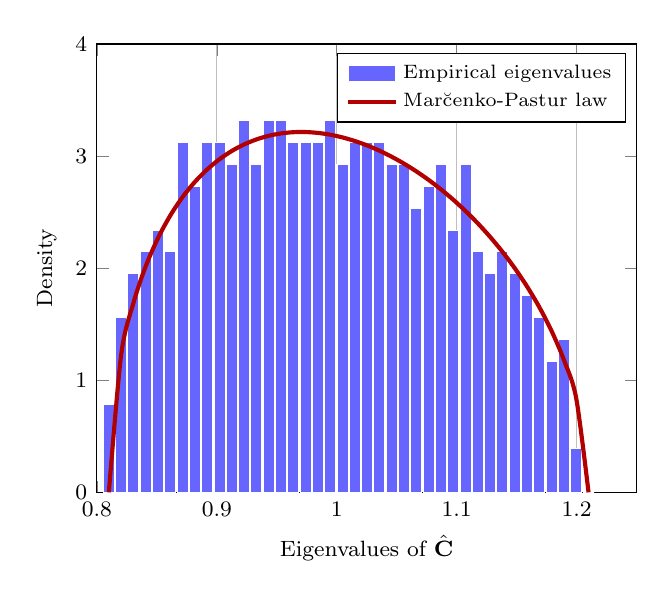
\begin{tikzpicture}[font=\footnotesize]
    \renewcommand{\axisdefaulttryminticks}{4} 
    %\pgfplotsset{every major grid/.append style={densely dashed}}       
    \pgfplotsset{every axis legend/.append style={cells={anchor=west},fill=white, at={(0.98,0.98)}, anchor=north east, font=\scriptsize }}
    \begin{axis}[
      %ybar,
      xmin=0.8,
      ymin=0,
      xmax=1.25,
      ymax=4,
      %xtick={0,1,2,3,4},
      % ytick={0,0.2,0.4,0.6,0.8},
      % yticklabels = {$0$,$0.2$,$0.4$,$0.6$,$0.8$},
      bar width=4pt,
      grid=major,
      ymajorgrids=false,
      scaled ticks=true,
      %scale ticks above={4},
      xlabel={Eigenvalues of $\hat \C$},
      ylabel={Density}
      ]
      \addplot+[ybar,mark=none,draw=white,fill=blue!60!white,area legend] coordinates{
      (0.810000, 0.780000)(0.820256, 1.560000)(0.830513, 1.950000)(0.840769, 2.145000)(0.851026, 2.340000)(0.861282, 2.145000)(0.871538, 3.120000)(0.881795, 2.730000)(0.892051, 3.120000)(0.902308, 3.120000)(0.912564, 2.925000)(0.922821, 3.315000)(0.933077, 2.925000)(0.943333, 3.315000)(0.953590, 3.315000)(0.963846, 3.120000)(0.974103, 3.120000)(0.984359, 3.120000)(0.994615, 3.315000)(1.004872, 2.925000)(1.015128, 3.120000)(1.025385, 3.120000)(1.035641, 3.120000)(1.045897, 2.925000)(1.056154, 2.925000)(1.066410, 2.535000)(1.076667, 2.730000)(1.086923, 2.925000)(1.097179, 2.340000)(1.107436, 2.925000)(1.117692, 2.145000)(1.127949, 1.950000)(1.138205, 2.145000)(1.148462, 1.950000)(1.158718, 1.755000)(1.168974, 1.560000)(1.179231, 1.170000)(1.189487, 1.365000)(1.199744, 0.390000)(1.210000, 0.000000)
      };
      \addlegendentry{{Empirical eigenvalues}}
      \addplot[smooth,RED,line width=1.5pt] plot coordinates{
      (0.810000, 0.000000)(0.820256, 1.226755)(0.830513, 1.690772)(0.840769, 2.017672)(0.851026, 2.269535)(0.861282, 2.471124)(0.871538, 2.635491)(0.881795, 2.770588)(0.892051, 2.881718)(0.902308, 2.972643)(0.912564, 3.046149)(0.922821, 3.104371)(0.933077, 3.148985)(0.943333, 3.181330)(0.953590, 3.202491)(0.963846, 3.213358)(0.974103, 3.214658)(0.984359, 3.206992)(0.994615, 3.190849)(1.004872, 3.166625)(1.015128, 3.134631)(1.025385, 3.095100)(1.035641, 3.048190)(1.045897, 2.993990)(1.056154, 2.932511)(1.066410, 2.863685)(1.076667, 2.787357)(1.086923, 2.703269)(1.097179, 2.611038)(1.107436, 2.510128)(1.117692, 2.399800)(1.127949, 2.279040)(1.138205, 2.146441)(1.148462, 2.000008)(1.158718, 1.836802)(1.168974, 1.652245)(1.179231, 1.438562)(1.189487, 1.180515)(1.199744, 0.838724)(1.210000, 0.000000)
      };
      \addlegendentry{{Mar\u{c}enko-Pastur law} }
    \end{axis}
  \end{tikzpicture}
  \caption{ Histogram of the empirical spectral distribution of $\hat \C$ versus the {Mar\u{c}enko-Pastur law, for $p=500$ and $ n= 50\,000$. }}
  \label{fig:MP-law}
\end{figure}

The elementary Mar{\u c}enko-Pastur result is already quite instructive and insightful.
\begin{remark}[When is one under the random matrix regime?]
Equation~\eqref{eq:MP-law} reveals that the eigenvalues of $\hat\C$, instead of concentrating at $x=1$ as a large-$n$ alone analysis would suggest, spread largely from $(1-\sqrt{c})^2$ to $(1+\sqrt{c})^2$. As such, for small $c$ (i.e., for large $n$), the eigenvalues span on a range
\begin{equation*}
    %(1+\sqrt{c})^2-(1-\sqrt{c})^2 = 4\sqrt{c} + O(c).
    (1+\sqrt{c})^2-(1-\sqrt{c})^2 = 4\sqrt{c}.
\end{equation*}
This is a slow decaying behavior. In particular, for $n=100p$, where one would expect a sufficiently large number of samples for $\hat \C$ to properly estimate $\C=\I_p$, $4\sqrt{c}=0.4$ which is a large spread around the mean (and true) eigenvalue $1$. This is visually confirmed by Figure~\ref{fig:MP-law} for $p = 500$ and $n = 50\,000$, where the histogram of the eigenvalues is nowhere near concentrated at $x=1$. As such, random matrix results will be largely more accurate than classical asymptotic statistics even when $n\sim 100p$. As a telling example, estimating the covariance matrix of each digit from the popular MNIST dataset \citep{lecun1998gradient}, made of no more than $60\,000$ training samples (and thus about $n=6\,000$ samples per digit) of size $p=784$, is likely a hazardous undertaking.
\end{remark}


\begin{remark}[On universality]\label{rem:universality}
Although introduced here in the context of Gaussian distributions for $\x_i$, the Mar{\u c}enko-Pastur law applies to much more general cases. Indeed, the result remains valid so long that the $\x_i$'s have i.i.d.\@ normalized entries of zero mean and unit variance (and even beyond this setting \citep{el2009concentration,louart2019concentration}). Similar to the law of large numbers in standard statistics, this \emph{universality} phenomenon commonly arises in random matrix theory and high dimensional statistics. We will exploit this phenomenon in the monograph to justify the wide applicability of the presented results, even to real datasets. 
\end{remark}



\subsection{Kernel matrices of large dimensional data}
\label{sec:intro-kernel}

\subsubsection{Main message}

Another less known but equally important example of the curse of dimensionality in machine learning involves the loss of relevance of the notion of Euclidean distance between large dimensional data vectors. To be more precise, we will see in the course of the manuscript that, \emph{under an asymptotically non-trivial classification setting} (that is, ensuring that asymptotic classification is neither too simple nor too hard), large and numerous data vectors $\x_1,\ldots,\x_n\in\RR^p$ extracted from a few-class mixture model tend to be asymptotically at equal distance from one another, irrespective of their mixture class. Roughly said, in this non-trivial setting and under reasonable statistical assumptions on the $\x_i$'s, we have
\begin{equation}\label{eq:distance-constant}
    \max_{1\leq i\neq j\leq n} \left\{ \frac1p\| \x_i - \x_j \|^2 - \tau \right\} \to 0
\end{equation}
for some constant $\tau$ as $n,p\to\infty$, \emph{independently of the classes (same or different) of $\x_i$ and $\x_j$} (here the distance normalization by $p$ is used for compliance with the notations in the remainder of the manuscript but has no particular importance).

This asymptotic behavior is extremely counter-intuitive and conveys the idea that classification by standard methods ought not be doable in this regime. Indeed, in the conventional finite-dimensional intuition that forged many of the leading machine learning algorithms of everyday use (such as spectral clustering \citep{ng2002spectral,von2007tutorial}), two data points belong to the same class if they are ``close'' in Euclidean distance. Here we claim that, when $p$ is large, \emph{data pairs are neither close nor far} from each other, regardless of their belonging to the same class or not. Despite this troubling loss of individual discriminative power between data pairs, we subsequently show that, thanks to a \emph{collective behavior} of all data belonging to the same (few and thus large) classes, asymptotic data classification or clustering is still achievable. Better, we shall see that, while many conventional methods devised from small dimensional intuitions do fail in the large dimensional regime, some popular approaches (such as the Ng-Jordan-Weiss spectral clustering method \citep{ng2002spectral} or the PageRank semi-supervised learning approach \citep{avrachenkov2012generalized}) still function. But the core reasons for their functioning are strikingly different from the reasons of their initial designs, and they often operate far from optimally.

\subsubsection{The non-trivial classification regime}

To get a clear picture of the source of Equation~\eqref{eq:distance-constant}, we first need to clarify what we refer to as the ``asymptotically non-trivial'' classification setting. Consider the simplest setting of a binary Gaussian mixture classification. We give ourselves a training set $\x_1, \ldots, \x_n \in \RR^p$ of $n$ samples independently drawn from the two-class ($\mathcal C_1$ and $\mathcal C_2$) Gaussian mixture
\begin{align*}
    % &\mathcal{C}_1: \x \sim \NN(\bmu, \I_p); \\
    % &\mathcal{C}_2: \x \sim \mathcal{N}(\zo, (1+\varepsilon)\I_p),
    &\mathcal{C}_1: \x \sim \NN(\bmu, \I_p); \\
    &\mathcal{C}_2: \x \sim \mathcal{N}(-\bmu, \I_p + \E),
\end{align*}
each drawn with probability $1/2$, for some deterministic $\bmu \in \RR^p$ and $\E \in \RR^{p \times p}$ both possibly depending on $p$. In the ideal case where $\bmu$ and $\E$ are perfectly known, one can devise a (decision optimal) Neyman-Pearson test. For an unknown $\x$, genuinely belonging to $\mathcal{C}_1$, the Neyman-Pearson test to decide on the class of $\x$ reads 
\begin{equation}\label{eq:NP-test}
    (\x + \bmu)^\T (\I_p + \E)^{-1} (\x + \bmu) - (\x - \bmu)^\T (\x - \bmu) \overset{\mathcal C_1}{\underset{\mathcal C_2}{\gtrless}} - \log \det(\I_p + \E).
\end{equation}
Writing $\x = \bmu + \z$ so that $\z \sim \NN (\zo, \I_p)$, the above test is equivalent to
\begin{align}
    %T(\x) \equiv \| \bmu \|^2 + 2\bmu^\T \z - \varepsilon \| \z \|^2 + p (1+\varepsilon) \log(1+\varepsilon) \overset{\mathcal C_2}{\underset{\mathcal C_1}{\gtrless}} 0.
    T(\x) \equiv& 4 \bmu^\T (\I_p + \E)^{-1} \bmu + 4 \bmu^\T (\I_p + \E)^{-1} \z + \z^\T \left( (\I_p + \E)^{-1} - \I_p \right) \z \nonumber \\
    %%
    &+ \log \det( \I_p + \E) \overset{\mathcal C_1}{\underset{\mathcal C_2}{\gtrless}} 0. \label{eq:NP-test-1}
\end{align}
Since $\U\z$ for $\U \in \RR^{p \times p}$ an eigenvector basis of $(\I_p + \E)^{-1}$ (and thus of $(\I_p + \E)^{-1} - \I_p$) follows the same distribution as $\z$, the random variable $T(\x)$ is the sum of $p$ independent random variables. Further assuming that $\|\bmu\|=O(1)$ with respect to $p$, by Lyapunov's central limit theorem (e.g., Theorem~27.3 in \citep{billingsley2012probability}), we have, as $p \to \infty$,
\begin{equation*}
    V_T^{-1/2} ( T(\x) - \bar T ) \cd \NN (0,1)
\end{equation*}
where
\begin{align*}
    % \bar T & \triangleq \| \bmu \|^2 - \varepsilon p + p (1+\varepsilon) \log(1+\varepsilon), \\
    % %%%
    % V_T & \triangleq 4 \| \bmu \|^2 + 2 \varepsilon^2 p.
    \bar T & \triangleq 4\bmu^\T (\I_p + \E)^{-1} \bmu + \tr (\I_p + \E)^{-1} - p + \log \det (\I_p + \E), \\
    %%%
    V_T & \triangleq 16 \bmu^\T (\I_p + \E)^{-2} \bmu + 2 \tr \left( (\I_p + \E)^{-1} - \I_p \right)^2.
\end{align*}
As a consequence, the classification performance of $\x \in \mathcal{C}_1$ is asymptotically non-trivial (i.e., the classification error neither goes to $0$ nor $1$ as $p \to \infty$) if and only if $\bar T$ is of the same order of $V_T^{-1/2}$. Considering the worst case scenario where $\E = \zo$, we must have $\| \bmu \| \geq O(1)$ with respect to $p$ (indeed, if instead $\| \bmu \|=o(1)$, the classification of $\x$ is asymptotically impossible).

%\footnote{This scaling is compatible with the following two situations
%\begin{enumerate}
%    \item $\bmu$ is delocalized, i.e., $\| \bmu \|_\infty = O(p^{-1/2})$;
%    \item $\bmu$ is sparse: it has a constant number of non-zero entries of magnitude $O(1)$.
%\end{enumerate}
%}
Under the minimal constraint of $\| \bmu \| = O(1)$ we move on to considering the case $\E \neq \zo$ with $\| \E \| = o(1)$. By performing a Taylor expansion of both $(\I_p + \E)^{-1}$ and $\log \det(\I_p + \E)$ around $\I_p$ we obtain
% \begin{equation*}
%     - \varepsilon p + p (1+\varepsilon) \log(1+\varepsilon) \geq O(1)
% \end{equation*}
\begin{align*}
    \bar T & = 4 \| \bmu \|^2  + \frac12 \tr (\E^2) + o(1); \\
    %%%
    V_T & = 16 \| \bmu \|^2 + 2 \tr (\E^2) + o(1),
\end{align*}
which demands $\tr(\E^2)$ to be of order $O(1)$ (as $\| \bmu \|$) so as to have discriminative power. Since $\tr (\E^2) \le p \| \E \|^2$, with equality if and only if $\E$ is proportional to identity, i.e., $\E= \epsilon \I_p$, one must have $\| \E \| \ge O(p^{-1/2}) $. Also, by the Cauchy–Schwarz inequality, we have $|\tr \E| \leq \sqrt{\tr (\E^2) \cdot \tr \I_p}=O(\sqrt{p})$, with equality if and only if $\E= \epsilon \I_p$, and we must therefore have $|\tr \E|\geq O(\sqrt{p})$. This allows us to conclude on the following non-trivial classification conditions
\begin{equation}\label{eq:non-trivial-conditions}
    \| \bmu \| \geq O(1), \quad \| \E \| \geq O(p^{-1/2}), \quad |\tr(\E)| \geq O(\sqrt{p}), \quad \tr(\E^2) \geq O(1).
\end{equation}
These are the minimal conditions for classification in the case of perfectly known means and covariances in the following sense: (i) if none of the inequalities hold (i.e., if means and covariances from both classes are too close), asymptotic classification must fail, (ii) if at least one of the inequalities is not tight (say if $\|\bmu\|\geq O(\sqrt p)$), asymptotic classification becomes trivial. 

\medskip

We shall subsequently see that \eqref{eq:non-trivial-conditions} precisely induces the asymptotic loss of distance discrimination raised in \eqref{eq:distance-constant} but that standard spectral clustering methods based on $n\sim p$ data remain valid.

\subsubsection{Asymptotic loss of pairwise distance discrimination}

Under the equality case for the conditions in \eqref{eq:non-trivial-conditions}, the (normalized) Euclidean distance between two distinct data vectors $\x_i \in \mathcal{C}_a, \x_j \in \mathcal{C}_b$ is thus given by
\begin{equation}\label{eq:distance-constant-concrete}
    \frac1p \| \x_i - \x_j \|^2 = \begin{cases} \frac1p \| \z_i - \z_j\|^2 + A p^{-1/2},  & \text{for} \ a=b=2; \\ \frac1p \| \z_i - \z_j\|^2 + B p^{-1/2}, & \text{for} \ a=1, b=2, \end{cases}
    %\| \bmu + \z_i - \sqrt{1+\varepsilon} \x_j \|^2
\end{equation}
where
\begin{align*}
    A & = \left( \z_i^\T \E  \z_i + \z_j^\T \E  \z_j - 2 \z_i^\T \E \z_j \right) p^{-1/2} \\
    %%%
    B &= \left( \z_j^\T ( \E + \E^2/4 ) \z_j - \z_i^\T \E \z_j + 4 \| \bmu \|^2 + 4 \bmu^\T (\z_i - \z_j) + o(1) \right) p^{-1/2}
\end{align*}
are both of order $O(1)$ and in particular $A > B$ with high probability for $p$ large, while the leading term $\frac1p \| \z_i - \z_j \|^2$ is of order $O(1)$ and such that
\begin{equation*}
    \max_{1\le i \neq j \le n} \left\{ \frac1p \| \z_i - \z_j \|^2 - 2 \right\} \to 0
\end{equation*}
almost surely as $n,p \to \infty$ (this easily follows by exploiting the fact that $\| \z_i - \z_j \|^2$ is a $\chi$-square random variable with $p$ degrees of freedom). As a consequence, as previously claimed,
\begin{equation*}
    \max_{1\le i \neq j \le n} \left\{ \frac1p \| \x_i - \x_j \|^2 - \tau \right\} \to 0
\end{equation*}
for $\tau=2$ here. Besides, let us suppose for the sake of argumentation that $\tr\E=0$ (a situation that arises for instance if the data entries $(\x_i)_k$ are variance-normalized). Then, on closer inspection of \eqref{eq:distance-constant-concrete}, beyond this common value $\tau$, the discriminative class information in means $4\|\bmu\|^2/p$ and in covariances $\z_j^\T\E^2 \z_j/(4p)\sim \tr \E^2/(4p)$ are both of order $O(p^{-1})$, while, by the central limit theorem, $\frac1p\|\z_i-\z_j\|^2=2+O(p^{-1/2})$. The class information is thus largely overtaken by the random fluctuations. As a consequence, asymptotically, $\frac1p \| \x_i - \x_j \|^2$ contains \emph{no} exploitable information (about $\bmu$ or $\E$) to distinguish if $\x_i$ and $\x_j$ vectors belong to the same or different classes.\footnote{For $\tr\E=O(p^{-1/2})$, the term $\frac1p\z_i^\T\E\z_i+\frac1p\z_j^\T\E\z_j\sim \frac2p\tr\E$ in $Ap^{-1/2}$ dominates $\frac1p\z_j^\T\E\z_j\sim \frac1p\tr\E$ in $Bp^{-1/2}$ and are both of order $O(p^{-1/2})$, which is the same order as the noise fluctuations. It is thus possible to non-trivially extract the class information in this case, in fact already from comparing the norms $\|\x_1\|,\ldots,\|\x_n\|$.}

\medskip

To visually confirm this joint convergence of the data distances, in Figure~\ref{fig:kernel-plot} we display the content of the radial basis function (RBF) kernel matrix $\K\in\RR^{n\times n}$ with $\K_{i,j} = \exp\left(-\frac1{2p} \| \x_i - \x_j \|^2 \right)$ and the associated second top eigenvector $\v_2$ for a two-class Gaussian mixture $\x \sim \NN (\pm \bmu, \I_p)$ with $\bmu = [2,\ \zo_{p-1}]$. For a constant $n=500$, we take $p=5$ in Figure~\ref{fig:kernel-plot-1} and $p=250$ in Figure~\ref{fig:kernel-plot-2}. 

While the ``block-structure'' in Figure~\ref{fig:kernel-plot-1} does agree with the finite-dimensional intuition that data vectors from the same class are ``closer'' to one another, corresponding to diagonal blocks with larger values (since $\exp(-x/2)$ decreases with the distance) than in non diagonal blocks, this intuition collapses when large dimensional data vectors are considered. Indeed, in the large data setting of Figure~\ref{fig:kernel-plot-2}, all entries (but obviously on the diagonal) of $\K$ have approximately the same value, which we now know from \eqref{eq:distance-constant} is $\exp(-1)$.

This is no longer surprising to us. However, what remains surprising at this stage of our analysis is that the eigenvector $\v_2$ of $\K$ is not affected by the asymptotic loss of class-wise discrimination of individual distances (particularly valid here since $\E=\zo$). Thus spectral clustering works equally well for $p=5$ or $p=250$, despite the radical and intuitively destructive change in the behavior of $\K$ for $p=250$.

\begin{figure}[htb]
\tikzset{
    position label/.style={
       below = 2pt,
       text height = 1.5ex,
       text depth = 1ex
    },
   brace/.style={
     decoration={brace, mirror},
     decorate
   }
}
    \begin{minipage}[c]{0.48\linewidth}
    \centering
    \[
        \v_2 = \left[\raisebox{-5pt}{
        \begin{tikzpicture}
      \begin{axis}[
      height=0.4\linewidth,
      width=1\linewidth,
      xmin=1,
      xmax=500,
      ymin=-.05,
      ymax=.05,
      hide axis
      ]
        \addplot [smooth,BLUE,line width=0.5pt] file {tikz/eig_vec_kernel1.txt};
    \end{axis}
    \end{tikzpicture}
    }\right]
    \]
    % \begin{tikzpicture}
    %     \node (C1start) at (0.5,0) {};
    %     \node (middle) at (2.8,0) {};
    %     \node (C2end) at (4,0) {};
    %     \draw [brace] (C1start.south) -- (middle.south) node [position label, pos=0.5] {$\mathcal{C}_1$};
    %     \draw [brace] (middle.south) -- (C2end.south) node [position label, pos=0.5] {$\mathcal{C}_2$};
    % \end{tikzpicture}
    \[
        \K = \left[\raisebox{-55pt}{
        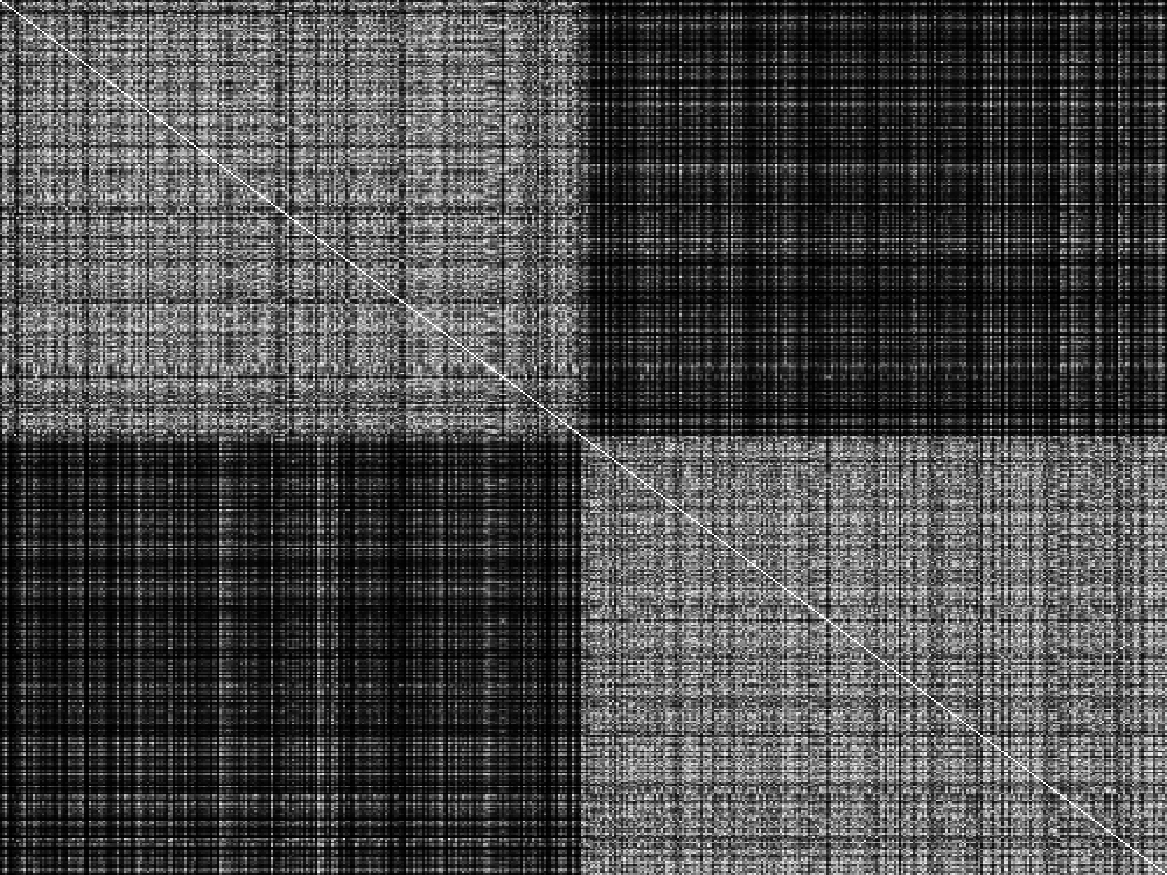
\includegraphics[width=.75\linewidth, height=.75\linewidth]{tikz/kernel1.png}
        % \begin{tikzpicture}
        % \begin{axis}[
        %     height = 1\linewidth,
        %     view={0}{90},
        %     axis equal image,
        %     colormap/blackwhite,
        %     hide axis
        % ]
        % \addplot3[matrix plot*] file {tikz/kernel1.dat};
        % \end{axis}
        % \end{tikzpicture}
        }
        \right]
    \]
    \subcaption{$p=5$, $n=500$.}\label{fig:kernel-plot-1}
    \end{minipage}
    \hfill{}
    \begin{minipage}[c]{0.48\linewidth}
    \centering
    \[
        \v_2 = \left[\raisebox{-5pt}{
        \begin{tikzpicture}
      \begin{axis}[
      height=.4\linewidth,
      width=1\linewidth,
      ymin=-.07,
      ymax=.07,
      xmin=1,
      xmax=500,
      hide axis
      ]
        \addplot [smooth,BLUE,line width=0.5pt] file {tikz/eig_vec_kernel2.txt};
    \end{axis}
    \end{tikzpicture}
    }\right]
    \]
    \[
        \K = \left[\raisebox{-55pt}{
        
\includegraphics[width=.75\linewidth, height=.75\linewidth]{tikz/kernel2.png}
        % \begin{tikzpicture}
        % \begin{axis}[
        %     height = 1\linewidth,
        %     view={0}{90},
        %     axis equal image,
        %     colormap/blackwhite,
        %     hide axis
        % ]
        % \addplot3[matrix plot*] file {tikz/kernel2.dat};
        % \end{axis}
        % \end{tikzpicture}
        }
        \right]
    \]
    \subcaption{$p=250$, $n=500$.}\label{fig:kernel-plot-2}
    \end{minipage}
    \caption{Kernel matrices $\K$ and the second top eigenvectors $\v_2$ for small and large dimensional data $\X = [\x_1,\ldots,\x_n] \in \RR^{p \times n}$ with $\x_1, \ldots, \x_{n/2} \in \mathcal{C}_1$ and $\x_{n/2+1}, \ldots, \x_n \in \mathcal{C}_2$.}
    \label{fig:kernel-plot}
\end{figure}

% {\RED *** J'aime bien l'idée qu'on prenne une approche "pitfalls/counterintuitive nature of large data". L'idée est de montrer que les choses se passent différemment en grandes dimensions et qu'on a vite fait de dire des bêtises. Deux exemples géniaux pour ça:
% \begin{itemize}
%     \item la matrice de cov empirique $XX'/n$ dont les entrées tendent bien vers $1$ sur la diag et $0$ en dehors (uniformément sur $p,n$! et même d'ailleurs si $n=p^m$) et donc donne l'impression qu'on tend vers une identité. Ce qui est vrai dans un sens (en norme infinie par exemple), mais PAS dans pour la norme opérateur qui est indispensable pour nous. On peut alors introduire MP, etc. de manière très intuitive, avec des dessins.
%     \item l'histoire du kernel. Là on peut expliquer facilement cette histoire des classes "non-triviales" en faisant du Neyman-Pearson sur $\mathcal N(\pm \mu,I_p)$ et $\mathcal N(0,(1+\varepsilon)I_p)$. On montre qu'il faut $\|\mu\|\geq O(1)$ et $|\varepsilon|\geq O(p^{-1/2})$. On montre alors que $\frac1p\|x_i-x_j\|^2\to$ constante dans ces conditions et on montre un dessin de la matrice à noyau dont toutes les entrées sont les mêmes, alors que... surprise le vep dominant contient les classes! (voir mes slides récents). 
% \end{itemize}
% Ce sont deux arguments géniaux pour montrer à quel point les choses se passent différemment en grandes dimensions et qu'il faut des outils pour comprendre tout ça. Dire alors que c'est {\bf là l'objectif du monographe}. ***}

\subsubsection{Explaining kernel methods with random matrix theory}

% {\BLUE *** Romain*** En fait, on a parlé avant de cov empirique, de ses problèmes et de la réponse apportée par RMT. Si ici, on parle de noyau, de ses problèmes, mais pas de la réponse apportée par RMT, on est inconsistents. Je préfère donc parler ici de ce que RMT fait. En plus, ça évite de revenir en arrière tout le temps sur des "bouts d'exemples" introduits plus tôt.}

The fundamental reason behind this surprising behavior lies in the \emph{accumulated} effect of the (in total) $n/2$ small ``hidden'' informative terms $\|\bmu\|^2$ and $\tr(\E^2)$, to collectively ``steer'' the several top eigenvectors of $\K$. More explicitly, we shall see in the course of this monograph that the RBF kernel matrix $\K$ can be asymptotically expanded as
\begin{align*}
    \K = \exp(-1) \left( \one_n \one_n^\T + \frac1p \Z\Z^\T \right) + g(\bmu,\E)\frac1p\j\j^\T + \ast + o(1)
\end{align*}
where $\Z=[\z_1,\ldots,\z_n]\in\RR^{p\times n}$, $g(\bmu,\E)=O(1)$ and $\j=[\one_{n/2}^\T,-\one_{n/2}^\T]^\T$ is the class-information vector (as in the setting of Figure~\ref{fig:kernel-plot}). Here `$\ast$' symbolizes extra terms of marginal importance to the present discussion and $o(1)$ represents terms of asymptotically vanishing \emph{operator} norm. The important remark to be made here is that
\begin{itemize}
    \item[(i)] under this description, $\K_{i,j}=\exp(-1)\left( 1 + \frac1p\z_i^\T\z_j \right)\pm \frac1pg(\bmu,\E)+\ast$ with $\frac1pg(\bmu,\E)\ll \frac1p\z_i^\T\z_j=O(p^{-\frac12})$: in consistent with our previous discussion that the information is \emph{entry-wise} dominated by noise;
    \item[(ii)] from a \emph{spectral} viewpoint, $\|\frac1p\Z^\T\Z\|=O(1)$, as per the Mar\u{c}enko-Pastur theorem \citep{marvcenko1967distribution} discussed in the previous section and $\|g(\bmu,\E)\frac1p\j\j^\T\|=O(1)$: thus, \emph{spectrum-wise}, the information stands on even ground with noise.
\end{itemize}
The key mathematical magic at play here lies in $g(\bmu,\E)\frac1p\j\j^\T$ having entries of order $O(p^{-1})$ but being a low rank (here unit rank) matrix: all its ``energy'' concentrates on a single eigenvalue. While for $\frac1p\Z^\T \Z$ with larger $O(p^{-1/2})$ amplitude entries, being composed of ``essentially independent'' zero mean random variables, it tends to \emph{spread} its energy over its $p$ eigenvalues. On comparison, both met on even ground ``somewhat'' under our aforementioned non-trivial classification setting. 

We shall see in Section~\ref{sec:kernel-methods} that things are actually not as clear-cut and in particular that not all kernel choices can reach the same (non-trivial) classification rates. Exceptionally, the popular Gaussian (RBF) kernel will be shown to be largely sub-optimal in this respect.

\subsection{Summarizing}

In this section we discussed two simple, yet counter-intuitive examples of common pitfalls in handling large dimensional data. 

In the sample covariance matrix example of Section~\ref{sec:intro-SCM}, we made the important remark of the loss of equivalence between matrix norms in the \emph{random matrix regime} where the data (or feature) dimension $p$ and their number $n$ are both large and comparable, which is at the source of many intuition errors. We in particular insist that, for matrices $\A_n,\B_n\in\RR^{n\times n}$ of large sizes
\begin{align}\label{eq:A_n-B_n}
    \forall i,j,~(\A_n-\B_n)_{i,j}\to 0 \not\Rightarrow \|\A_n-\B_n\|\to 0
\end{align}
in operator norm.

We also realized, from a basic reading of the Mar\u{c}enko-Pastur theorem, that the random matrix regime arises more often than one may think: while $n/p \sim 100$ may seem large enough a ratio for classical asymptotic statistics to be accurate, random matrix theory is in general a far more appropriate tool (with as much as $20\%$ gain in precision for the estimation of the eigenvalues of sample covariances). 

In Section~\ref{sec:intro-kernel}, we gave a concrete machine learning classification example of the message \eqref{eq:A_n-B_n} above. We saw that, in the practically most relevant scenario of non-trivial (not too easy, not too hard) large data classification tasks, the distance between any two data vectors ``concerntrates'' around a constant \eqref{eq:distance-constant}, regardless of their respective classes. Yet, since again $(\A_n)_{i,j}\to\tau$ does not imply that $\|\A_n-\tau \one_n \one_n^\T\|\to 0$ in operator norm, we understood that, thanks to a collective effect of the small but similarly ``oriented'' fluctuations, spectral clustering remains valid for large dimensional problems. 

\medskip

Possibly most importantly, we discovered that the curse of dimensionality induced by the eerie behavior of large dimensional vectors turns into an asset for mathematical analysis. In the sample covariance matrix example, we observed a random-matrix version of the laws of large numbers arises in the convergence to a deterministic limit of the eigenvalue distributions of large sample covariance matrices. As a matter of fact, as we shall see throughout the monograph, the very fact that both $p$ and $n$ are large ensures a generally \emph{fast convergence} of most quantities of practical interest: by exploiting $np=O(n^2)$ rather than $n$ degrees of freedom, central limit theorems may converge at $O(1/n)$ speed (instead of the classical $O(1/\sqrt{n})$). 

This fast convergence further induces another important phenomenon, referred to as the \emph{universality} which ensures the robustness of the random matrix asymptotics to a vast range of distributions. Essentially, as we shall see in more details later in this monograph, first and second order statistics are often sufficient to describe most asymptotic behaviors, even of complicated data models and methods. This is a first (yet not the most convincing) justification of the repeatedly observed strong match between random matrix predictions and practical simulations on real datasets.

\medskip

In a nutshell, the fundamental counter-intuitive yet mathematically addressable changes in behavior of large dimensional data have two major consequences to statistics and machine learning: (i) most algorithms, originally developed under a finite-dimensional intuition, are likely to fail (as we shall discover in this monograph, many of them do) or at least to perform inefficiently, yet (ii) by benefiting from the extra degrees of freedom offered by large data, random matrix theory is apt to analyse, improve, and evoke a whole new paradigm for large dimensional learning.


\section{Random matrix theory as an answer}

\subsection{Which theory and why?}

\subsubsection{A point of history}
Random matrix theory originates from the work of John Wishart \citep{wishart1928generalised} on the study of the eigenvalues of the matrix $\X\X^\T$ (now referred to as a Wishart matrix) for $\X\in\RR^{p\times n}$ with $\X_{i,j}\sim\NN(0,1)$. Wishart managed to determine a closed-form expression for the joint eigenvalue distribution of $\X\X^\T$ for every pair $p,n$. Few progress however followed, as matrices with non-Gaussian entries are not amenable to this analysis and, even if they were, the actual study of more elaborate functionals of $\X\X^\T$ is at best cumbersome and often simply intractable.

The works of the physicist Eugene Wigner \citep{wigner1955characteristic} gave a new impulse to the theory. Interested in the eigenvalues of symmetric matrices $\X\in\RR^{n\times n}$ with independent Bernoulli entries (spins), Wigner opted for an \emph{asymptotic} analysis of the eigenvalue distribution, thereby initiating the important and much richer branch of \emph{large dimensional random matrix theory}. Despite this important inspiration, Wigner exploited standard asymptotic statistics tools (the method of moments) to prove that the \emph{discrete} distribution of the eigenvalues of $\X$ has a \emph{continuous} semi-circle looking density in the limit (the now popular semi-circular law). This approach was particularly convenient as the limiting law is simple and could be visually anticipated. 

Only in 1967 with the tour-de-force of Mar\u{c}enko and Pastur \citep{marvcenko1967distribution} did random matrix theory take a new dimension. Mar\u{c}enko and Pastur determined the limiting spectral distribution of the sample covariance matrix model $\X\X^\T$ of Wishart but under relaxed conditions: $\X_{i,j}$ are independent entries with zero mean and unit variance, with no further assumption. The independence (or weak dependence) property is key to this method. The proof exploits the powerful Stieltjes transform $\frac1p\tr(\frac1n\X\X^\T-z\I_p)^{-1}$ of the empirical spectral distribution of $\frac1n\X\X^\T$, a tool borrowed from operator theory in Hilbert spaces \citep{akhiezer2013theory}, rather than the moments $\frac1p\tr (\frac1n\X\X^\T)^k$ (which may not converge since $\EE[\X_{i,j}^\ell]$ needs not be finite for $\ell>2$). 

The technical approach devised by Mar\u{c}enko and Pastur was then largely embraced at the turn of the 21st century by Bai and Silverstein who, in a series of significant breakthroughs \citep{silverstein1995empirical,bai1998no}, extended \citep{marvcenko1967distribution} to an exhaustive study of sample covariance matrices.

In parallel, another approach to limiting spectral analysis of random matrices emerged as an application example of the \emph{free probability theory} developed by Voiculescu \citep{voiculescu1992free}. Free probability was born as a theory to study random variables in non-commutative algebras, such as the algebra of matrices. Rather than relying on independence assumptions as for the Stieltjes transform method, free probability relies on a notion of \emph{asymptotic freeness}. In essence, random matrices are asymptotically free if their eigenvector distribution are sufficiently isotropic with respect to each other; for instance, independent Gaussian matrices (matrices with independent Gaussian entries) are free, independent unitary matrices with isotropic eigenvector distributions are free, a deterministic matrix is free with respect to a Gaussian matrix, etc. 

Both free probability and the Stieltjes transform approach have long lived hand-in-hand, and are essentially capable of proving similar results under various assumptions. A classical example, of great importance to this monograph, is that of \emph{spiked models} (i.e., finite-rank deformation of random matrices, such as the non-zero mean sample covariance $(\X+\bmu \one_n^\T)(\X+\bmu \one_n^\T)^\T$ for $\X$ with i.i.d.\@ centered entries and mean vector $\bmu \in\RR^p$) made popular by two key articles \citep{baik2006eigenvalues} and \citep{benaych2012singular}, respectively based on a Stieltjes transform and a free probability approach.

These tools are largely sufficient to cover most of the basic statistical problems in random matrix theory. In particular, the often called \emph{global regime} of random matrices: their limiting eigenvalue spectrum, the behavior of linear statistics of their eigenvalues or eigenvectors, the position of the outlying eigenvalues in spiked models, etc., are all amenable to study by either method. However, this is often not the case of the \emph{local regime}: the limiting distribution of a specific eigenvalue (notably the largest and smallest of practical interest) cannot be study by these methods. There, researchers have rather resorted to a finite dimensional analysis of the joint eigenvalue distribution for the Gaussian case (in the spirit of Wishart), and carefully taken the limits of the distribution, exploiting powerful tools in orthogonal polynomial theory \citep{johnstone2001distribution}. We will not further discuss this approach in the monograph, which is too specific and not of direct use to our applications.

\subsubsection{Resolvents, Gaussian tools, and concentration of measure theory}
More recently, the attractivity of the free probability approach decayed, as asymptotic freeness no longer holds for structured random matrix models of importance for application purposes. For this very reason, our focus in this monograph will be on the range of methods surrounding the Stieltjes transform approach. 

Precisely, our central object of study throughout the monograph is the so-called \emph{resolvent} of the random matrix $\X\in\mathbb{R}^{n\times n}$ under investigation, that we shall often denote $\Q_\X(z)$ or simply $\Q(z)$, and that is defined, for all $z\in\CC$ not in the spectrum of $\X$, by
\begin{align*}
    \Q_\X(z) \equiv \left( \X - z\I_n \right)^{-1}.
\end{align*}
The resolvent is a rich mathematical object that gives access to 
\begin{itemize}
    \item \emph{the eigenvalue distribution} $\mu_\X\equiv \frac1n\sum_{i=1}^n\delta_{\lambda_i(\X)}$ of $\X$ through the Stieltjes transform relation (for all $a,b\notin \{\lambda_1(\X),\ldots,\lambda_n(\X)\}$)
\begin{align*}
    \int_a^b \mu_\X(d\lambda) &= \lim_{\varepsilon\to 0^+} \int_a^b \frac1\pi \Im[m_\X(x+i\varepsilon)]dx \\
    m_\X(z) &\equiv \int \frac{\mu_\X(d\lambda)}{\lambda-z} = \frac1n\tr\Q_\X(z)=\frac1n\sum_{i=1}^n\frac1{\lambda_i(\X)-z};
\end{align*}
    \item \emph{functionals of these eigenvalues} $\frac1n\sum_{i=1}^nf(\lambda_i(\X))$ through the Cauchy's integral identity 
    \begin{align*}
        \frac1n\sum_{i=1}^nf(\lambda_i(\X)) &= -\frac1{2\pi\imath n}\oint_{\Gamma} f(z)\tr(\Q_\X(z))dz
    \end{align*}
    for $\Gamma\subset \CC$ a positively oriented contour surrounding all the $\lambda_i(\X)$'s and $f(z)$ complex analytic in a neighborhood of the inside of $\Gamma$;
    \item \emph{the eigenvectors and subspaces} of $\X$, again through Cauchy's integral relation
    \begin{align*}
        \uu_i(\X)\uu_i(\X)^\T &= -\frac1{2\pi\imath}\oint_{\Gamma_{\lambda_i(\X)}} \Q_\X(z)dz
    \end{align*}
    for $(\lambda_i(\X),\uu_i(\X))$ an eigenpair of $\X$ and $\Gamma_{\lambda_i(\X)}$ a positively oriented contour surrounding only $\lambda_i(\X)$.
\end{itemize}
In addition, the resolvent is a natural object that frequently appears in the solutions to linear regression problems (for machine learning applications, in least-square support vector machines, extreme learning machines, echo-state neural networks, etc.) or to random walk and graph-based semi-supervised learning methods. They will also be shown to appear naturally in not immediately related machine learning problems, such as in large dimensional nonlinear regression (logistic or robust M-regression).

\bigskip

The core of the random matrix approach devised in this monograph consists in determining, for various statistical models of matrices $\X$ a \emph{deterministic equivalent} $\bar\Q(z)$ for $\Q(z)=\Q_\X(z)$, in the sense that
\begin{align*}
    u(\Q(z)-\bar\Q(z))\asto 0,\quad \textmd{or}\quad u(\EE[\Q(z)]-\bar \Q(z))\to 0
\end{align*}
for all $1$-Lipschitz linear application $u:\RR^n\to \RR$. Of particular interest are the functions $u(\Z)=\frac1n\tr (\A\Z)$ for $\|\A\|\leq 1$, $u(\Z)=\a^\T\Z\b$ for $\|\a\|,\|\b\|\leq 1$.

As an example, in the setting of the Mar\u{c}enko-Pastur law where the random matrix of interest is $\frac1n\X\X^\T$ with $\X$ having i.i.d.\@ zero mean and unit variance entries,
\begin{align*}
    \Q(z) = \left( \frac1n\X\X^\T - z\I_p \right)^{-1}
\end{align*}
admits
\begin{align*}
    \bar\Q(z) = m_\mu(z) \I_p,\quad m_\mu(z)=\int\frac{\mu(d\lambda)}{\lambda-z},\quad \mu\textmd{ defined in }\eqref{eq:MP-law}
\end{align*}
as deterministic equivalent. Thus, in particular, $\frac1n\tr \Q(z)-m_\mu(z)\asto 0$ and $\a^\T\Q(z)\b - m_\mu(z)\a^\T\b \asto 0$ for all $\a,\b$ of bounded norm.

\bigskip

In order to determine and investigate these deterministic equivalents, tools from three main mathematical areas are required:
\begin{itemize}
    \item \emph{linear algebra}, mostly in the exploitation of inverse matrix lemmas, the Schur complement, interlacing and low rank perturbation identities \citep{horn2012matrix};
    \item \emph{complex analysis} (the resolvent $\Q(z)$ is a complex analaytic matrix-valued function) and particularly the theory of analytic functions, contour integrals and residue calculus;
    \item \emph{probability theory}, and particularly notions of convergence, central limit theory, moment methods, etc.\@ \citep{billingsley2012probability}. More specifically, depending on the underlying random matrix assumptions (independence of entries, Gaussianity, concentration properties), different random matrix-adapted techniques will be discussed: the Gaussian tools developed by Pastur, relying on Stein's lemma and the Nash-Poincaré inequality \citep{pastur2011eigenvalue}, the Bai-Silverstein inductive method \citep{bai2010spectral}, the concentration of measure framework developed by Ledoux \citep{ledoux2001concentration} and applied to random matrix endeavours successively by El Karoui, Vershynin, and Louart in \citep{el2009concentration,vershynin2010introduction,louart2019concentration}, or the double leave-one-out approach devised by El-Karoui in \citep{el2013robust}.
\end{itemize}
In a nutshell, all aforementioned methods are perturbation methods in the sense that they exploit the fact that, by eliminating a row or column (say here both row and column $i$) of $\X$ to obtain $\X_{-i}\in\mathbb{R}^{(n-1)\times (n-1)}$, the resolvent $\Q_{-i}(z)=(\X_{-i}-z\I_{n-1})^{-1}$ can be related to the original resolvent $\Q(z)$ through both linear algebraic relations and asymptotically comparable statistical behaviors. For instance, in the case of symmetric $\X$ with i.i.d.\@ (properly normalized) entries, it is not difficult to show that $m_\X(z)=m_{\X_{-i}}(z)+O(n^{-1})$.

In this regard, Pastur's Gaussian method manages, for models of $\X$ involved Gaussianity, to obtain asymptotic relations of $\EE[\Q(z)]$. Interpolation methods may then be used to extrapolate the results beyond the Gaussian case. The Bai-Silverstein inductive method is not restricted to matrices of Gaussian entries but is restricted to the specific analysis of either trace forms $\tr (\A\Q(z))$ or bilinear forms $\a^\T\Q(z)\b$ that need be treated individually. The concentration of measure approach is quite versatile: by merely restricting the matrix under study to be constituted of \emph{concentrated random vectors} (so in particular, Lipschitz maps of standard Gaussian random vectors or of vectors with i.i.d.\@ entries), it allows to study $\EE[\Q(z)]$ directly as well.
%in its columns

\subsection{The double asymptotics: turning the curse of dimensionality to a dimensionality blessing}

The major technical difficulty that has long held many machine learning away from tractable analysis and theoretical comprehension relates to the non-linearity involved in feature extraction (nonlinear kernels, nonlinear activation functions in neural networks), to the implicit nature of some methods (such as for the popular logistic regression), and eventually to the difficulty of a proper (statistical) modeling for arbitrary data (starting with images). 

An all-encompassing example of these difficulties could be summarized as the following problem: 
\smallskip

\noindent\fbox{\parbox{.98\linewidth}{
{\bf Problem.} Determine the classification performances of logistic regression for $n$ observations of $p$-dimensional random feature vectors extracted from a set of two-class images (say, images of dogs versus images of cats).
}}

\smallskip

In the conventional wisdom of machine learning research, one cannot conceive to solve this problem: the input data (real images) cannot be easily modelled, the nonlinear features extracted from those data are complex mathematical objects (even in the case where the original data could be modelled as simply as Gaussian vectors), and the logistic regression is an implicit optimization method not amenable to mathematical analysis. {\BLUE not easily amenable to mathematical analysis for a direct exposure of the classification performances.}
{\RED *** Je ne comprends pas ta phrase. Ça veut dire quoi "explicit exposure" ? ***}
{\BLUE C'est mieux avec "direct exposure"? En fait je trouves cette partie en peu agressive... Dans les edtudes de statistical learning theory "classique", on SAIT comment traiter la nonlinearite (avec les bornes ou RKHS etc), je penses il faut faire un peu plus modeste et dire qu'on a les perf plus precise et explicit avec RMT.}

We shall demonstrate throughout this monograph that random matrix theory provides a satisfying answer to all these difficulties at once and can actually \emph{solve} the Problem. This is made possible by the powerful joint \emph{universality} and \emph{determinism} effects brought by large dimensional data models and treatments.

Specifically, in the random matrix regime where $n,p$ grow large at a controlled rate, the following key properties arise:
\begin{itemize}
    \item \emph{fast asymptotic determinism}: the law of large numbers and the central limit theorem tell us that the average of $n$ i.i.d.\@ random variables converges to a deterministic limit at a $O(1/\sqrt{n})$ speed. By gathering independence (or degrees of freedom) both in the sample dimension $p$ and size $n$, functionals of random matrices (even complex functionals, such as the average of functions of their eigenvalues) also converge to deterministic limits, but at an increased speed of up to $O(1/\sqrt{np})$ which, for $n\sim p$, is $O(1/n)$. In machine learning, performances may be expressed in terms of correct classification rates (i.e., averaged statistics of sometimes involved random matrix functionals) and can thereby be predicted with high accuracy, even for not too large dimensional datasets;
    \item \emph{universality}: similarly, again consistently with the law of large numbers and the central limit theorem in the large $n$ alone setting, the above asymptotic deterministic behavior at large $n,p$ is in general independent of the underlying distribution of the random matrix entries. This phenomenon, referred to in the random matrix literature as \emph{universality}, predicts notably that the asymptotic statistics of even complex machine learning procedures only depend on first and second order statistics of the input data;
    \item \emph{linearization behavior}: the above properties explain that linear statistics are asymptotically predictable. What additionally appears in the large $n,p$ regime is that, due to concentration of even elementary objects (such as distances $\|\x_i-\x_j\|$ previously discussed), the functioning points of many algorithms moves from continuous to discrete and finite. In the kernel random matrix example, only the derivatives of the kernel function $f$ at $\tau$ matter. In random neural networks, all the information will be encapsulated in a single deterministic matrix involving the random distribution of the hidden layers and the activation function. In implicit optimization schemes (such as logistic regression), the solution ``concentrates'' with predictable asymptotics which, despite the initial non-linear convex optimization problem, only depend on first order statistics;
    \item \emph{tractable real data modelling}: possibly the most important aspect though relates to the counter-intuitive fact that, as $p,n$ grow large, machine learning algorithms tend to treat real data as if they were mere Gaussian mixture models. This statement, discussed thoroughly in the subsequent sections, is both sustained by empirical observations (most theoretical findings tend to fit with performances on real data) and by the theoretical fact that some extremely realist datasets (in particular artificial images created by generative adversarial networks) are by definition \emph{concentrated random vectors} which are (i) amenable to random matrix analysis, (ii) proved to behave as if mere Gaussian models.
\end{itemize}
In a nutshell, in large dimensions, data do not really ``spread'' all over their large ambient space but, by accumulation of degrees of freedom, rather concentrate in a thin lower-dimensional layer. Each scalar observation of the data, even by complicated functions (regressors, classifiers for us), then tends to become deterministic, predictable and simple functions of first order statistics. Random matrix theory exploits these effects and is thus capable to answer seemingly challenging machine learning questions.


%{\RED *** J'ai peur que cette section soit trop redondante avec ce qu'on a déjà dit et/ou aille trop loin déjà. Je dois y réfléchir... ***}



%The conventional wisdom to handle nonlinear systems and functions is to perform a (local) \emph{linearization}, for example via a Taylor expansion. This is widely used in the stability analysis of dynamical systems \citep{arrowsmith1992dynamical} and in statistics under the name of Delta method \citep{van2000asymptotic}. Taking again the example of (translation invariant) kernel matrix as in Section~\ref{sec:intro-kernel} with
%\begin{equation}\label{eq:intro-kernel-matrix}
%    \K_{i,j} = f \left( \frac1p \| \x_i - \x_j \|^2 \right)
%\end{equation}
%for some nonlinear function $f:\RR \mapsto \RR$ (e.g., $f(x) = e^{-x/2}$ in the case of RFB kernel). The curse of dimensionality in \eqref{eq:distance-constant} now becomes a ``dimensionality blessing'', which allows us to perform a Taylor expansion of the nonlinear function $f(x)$ (that shall be assumed to be differentiable for the moment) around $x = \tau$ and to obtain the following (asymptotic) linearization
%\begin{equation}\label{eq:intro-K-approx}
%    \| \K - \tilde \K \| \asto 0, \quad \tilde \K = \frac{C}p \Z^\T \Z + \J \A \J^\T + *
%\end{equation}
%as $n,p \to \infty$, where $\Z = [\z_1, \ldots, \z_n] \in \RR^{p \times n}$, $C$ some deterministic constant depending on $f$, $\J = [\j_1, \j_2] \in \RR^{n \times 2}$ with $\j_a$ the canonical vector of class $\mathcal{C}_a$ such that $(\j_a)_i = \delta_{\x_i \in \mathcal{C}_a}$ and $\A$ contains the statistical ``information'' $\bmu, \E$ of the data.

%As such, we obtain an \emph{asymptotic equivalent} $\tilde \K$ of the nonlinear kernel matrix $\K$ defined in \eqref{eq:intro-kernel-matrix}. They are equivalent in the sense that the operator norm of their difference goes almost surely to zero as $n,p \to \infty$. As discussed in Remark~\ref{rem:operator-norm}, this provides access to the eigenspectrum, the isolated eigenvalues/eigenvectors (based upon which spectral clustering is performed), as well as many other \emph{linear functionals} of $\K$ (e.g., the regression vectors or label/store vectors for classification), by studying those of the equivalent $\tilde \K$ that is more tractable.

%It is also of interest to note that, despite the pairwise loss of distance discrimination in \eqref{eq:distance-constant}, Equation \eqref{eq:intro-K-approx} above entails a ``collective conservation'' of the discriminative power of $\K$ at a matrix level, since $\tilde \K$ indeed contains $\J \A \J^\T$ which reflects the structural information of the dataset $\X$. This explains why spectral clustering may (possibly) work, with a wise choice of $f$ on function of the data statistics $\bmu,\E$, in the large $n,p$ regime. In fact, similar to the case of $n \to \infty$ alone with $p$ fixed where the diversity of the number of data provides convergence through laws of large numbers, taking into consideration the fact that $p$ is also large helps establish convergence of some key objects (e.g., $\K_{i,j}$) by exploiting the diversity offered by the size of each data/feature vector, so that the assessment of (e.g., the performance of) machine learning algorithms become technically more accessible. Moreover, this ``double-asymptotics'' regime also benefits in terms of convergence rate, since there are in total $np = O(n^2)$ independent random variable, the rate of convergence can, in the best case, be up to $O(n)$ which is much faster than the $O(\sqrt{n})$-rate offered by the central limit theorem in the large-$n$ alone case.

% {\RED
% *** Ici, on parle des difficultés de traiter les problèmes de ML (non-linéarité des méthodes, solutions implicites de problèmes d'optim, applications à des vraies données là où on ne sait que traiter des problèmes statistiques simples (au mieux mélanges de gaussiennes!). On boucle alors avec la partie précédente: déjà qu'on ne sait pas estimer correctement la covariance population, quels désastres cela crée-t-il sur les méthodes utilisées tous les jours? On montre alors que RMT apporte la solution et qu'{\bf en plus}, en exploitant des degrés de libertés supplémentaires, on résoud tous ces problèmes. ***

% *** On explique alors la méthode qu'on suit pour traiter les problèmes:
% \begin{itemize}
%     \item quand on a des modèles non linéaires: on trouve un équivalent aléatoire asymptotique qu'on sait manipuler. On donne ici l'exemple du noyau $K$ sous une forme très très simple, e.g., $K\simeq ZZ'+JAJ'+*$
%     \item une fois ramené à un modèle aléatoire à entrées indépendantes, on utilise les outils de la RMT: méthode de la résolvante, intégrales de contour, etc. pour identifier le spectre, les vaps isolées, le contenu des veps, et, {\bf plus important}, étudier les fonctionelles linéaires des matrices aléatoires (les scores de classif, la valeur des régressions, les classes attribuées par le clustering, etc.).
% \end{itemize}
% }


\subsection{Improving machine learning methods}

{\RED 
*** Là on dit que l'analyse précédente donne la possibilité de comprendre les limitations et d'améliorer les perfs / donner de nouvelles intuitions pour changer les algos ML. L'exemple SSL de Xiaoyi est particulièrement génial pour ça, on peut le détailler ici. ***}

{\BLUE 
En fait, j'ai pas trop idee comment introduire l'histoire de SSL ici, il faut parler de: 1. le probleme de SSL; 2. le soucis de "pas utiliser les donnees labelisees" en grande dimension et 3. pourquoi avec PKP on resout ce probleme. J'ai l'impression c'est un peu dense dans l'intro ici.
}

{\RED
*** Là mon idée est vraiment qu'on fasse un plan de la suite du bouquin, mais pas un plan "classique", grand I, grand II, etc., plutôt une approche cohérente: on part d'outils mathématiques (eq dét de la résolvante par exemple) qu'on étudie, ces objets sont au coeur de plein d'algos de ML, on arrive à les analyser. On comprend alors ce qu'ils font, pourquoi on comprend que les algos les plus utilisés sont ceux-ci ou ceux-là (les autres ne marchent pas, et on le prouve!), on montre alors qu'ils ne sont pas optimaux, et on peut les améliorer. Tout ça c'est valable pour à peu près tout ce qu'on a fait. ***
}



\subsection{Exploiting universality: from large dimensional statistics to practical data}

{\RED *** Ici, du coup, on s'appuie sur ce qu'on a dit avant, mais qui est basé sur des études de mélanges gaussiens souvent. On dit que bizarrement ça colle bien avec ce qu'on voit pour des vraies données. La question est de savoir: en quoi ces vraies données sont si "proches" d'un comportement gaussien. Et là on déballe notre sauce, avec l'histoire des GANs ***}

In this section, we further elaborate on the universality phenomenon briefly discussed in the previous sections, which carries a much deeper importance than one may anticipate.

\bigksip

First, let us recall that most random matrix results derived in the literature, even the most recent on machine learning applications (mostly discussed in this monograph), are based on the assumption of data arising either from Gaussian (possibly mixture) distributions or represented by vectors with independent entries. These vector distributions are naturally deemed unrealistic models for realistic data and we will not claim otherwise. It is a fact that real data, such as images, are largely more complex than mere Gaussian vectors.

Yet, what we do claim, is that \emph{scalar observations} (regression or classifier outputs, misclassification rates, etc.) obtained from large data or large datasets \emph{tend to behave as if the data were Gaussian} (mixtures) in the first place. This is a fundamental rupture that random matrix theory structurally exploits: rather than assuming data as fixed entities living in a complex manifold, random matrix theory mostly exploits their numerous degrees of freedom which, by universality, induce deterministic behavior in the large dimensional limit.

We justify this claim below with two strong arguments: one empirical and one theoretical.

\bigskip

Our first argument follows after numerous comparative experiments made between theoretical findings on Gaussian datasets versus real datasets. Indeed, although mostly derived under simple and unrealistic Gaussian mixture models, many theoretical results mentioned above show an \emph{unexpected close match} when applied to popular real-world large dimensional datasets, such as the MNIST handwritten-digit dataset \citep{lecun1998gradient}, the related Fashion-MNIST data \citep{xiao2017fashion}, the German Traffic Sign dataset \citep{houben2013German}, as well as numerous financial and electro-encephalography (EEG) time series data. To be more precise, ...

%%%%

As already mentioned in Remark~\ref{rem:universality}, this surprising accordance between theory and practice is possibly due to the \emph{universality} of random matrix theory results, i.e., only the first several moments matter in determining the asymptotic behavior of the eigenspectrum, as in the case of Mar{\u c}enko-Pastur law. 


However, recent advances in \emph{concentrated random vectors} \citep{el2009concentration,louart2019concentration} provide the possibility to go even beyond this setting. Consider a random vector $\x \in \RR^p$, we say it is \emph{concentrated} if, for all Lipschitz function $f: \RR^p \mapsto \RR$, there exists deterministic $m_f \in \RR$ such that
\begin{equation*}
    P \left( | f(\x) - m_f | > \epsilon \right) \le e^{-g(\epsilon)}
\end{equation*}
for some strictly increasing function $g: \RR \mapsto \RR$. Intuitively speaking, a concentrated random vector can be seen as a (random) point in the high dimensional space that, through any ``observation'' $f$ that maps the given point to the ``observable world'' $\RR$, always exhibits a ``similar'' and tractable behavior in the sense that, with high probability, the random variable $f(\x)$ takes values very close to the deterministic $m_f$ so that in the ``observable world'', the observation $f$ (which can typically be any performance metrics of the machine learning algorithm on a new test data $\x_i$) appears to be ``stable'' for any concentrated $\x_i$. 

Although there is no reason to assume real data (for example real images) are concentrated random vectors, it turns out to be \emph{almost} the case, due to the success of generative adversarial networks (GANs) \citep{goodfellow2014generative,brock2018large}. GANs generate ``artificial'' images from random Gaussian (and thus concentrated) vectors by passing them through a layered structure with entry-wise non-linearity, which indeed forms a Lipschitz mapping. The output image vectors (as those in Figure~\ref{fig:biggan}) are thus also concentrated vectors (according to ??), while it’s almost impossible to tell that they’re not real images, even for human beings. As such, concentrated random vectors appear to be \emph{ideal} for modelling real-world data, at least in handling real images data.


\begin{figure}[htb]
    \centering
    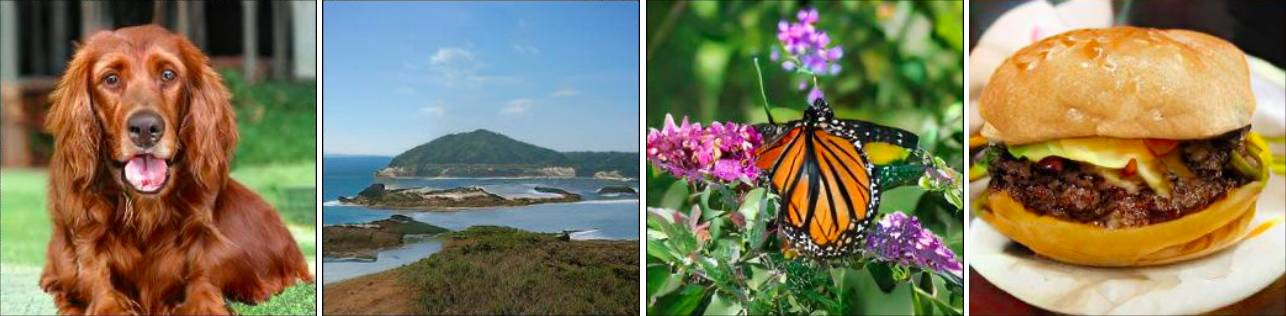
\includegraphics[width=.85\linewidth]{BigGan.jpg}
    \caption{Images samples generated by BigGAN in \citep{brock2018large}}
    \label{fig:biggan}
\end{figure}

{\RED 
*** Là je propose qu'on dise que les méthodes décrites ci-dessus marchent étonnament bien pour des vraies données (on donne des exemples sur MNIST / German signs, etc.). On parle alors d'universalité de la RMT: les résultats sont vraies au premier ordre indépendamment de la loi des entrées iiid. MAIS, il faut alors dire qu'on se limite à des vecteurs iid, ce qui est un problème en pratique. On dit alors qu'on peut faire tout ça en vecteurs concentrés et on montre l'exemple des GANs et de la prédiction fine pour des vraies données. ***

*** Tout ça devrait faire une très bonne intro! ***

}


\section{Organization of the manuscript}
\label{sec:organization}

{\RED 

\section{Some notations and basic notions}

}

Stochastic convergence:
\begin{itemize}
	\item convergence weakly = convergence in distribution (pointwise convergence of the distribution function in all continuity points of the limit distribution).
	\item convergence in probability: $\lim_{n \to \infty} P(|x_n - x| > \varepsilon) = 0$ for all $\varepsilon > 0$. which can be further extend to a convergence in probability of $f(x_n)$ to $f(x)$ for every continuous function $f$, as a result of the continuous mapping theorem.
	\item almost sure convergence or convergence with probability one: $P(\lim_{n \to \infty} x_n = x) = 1$, this is the strongest convergence and can be usually proved with Borel-Cantelli lemma.
	\item convergence in probability $\Rightarrow$ weak convergence, the converse is generally wrong but is true in the case of a weak convergence to a constant.
\end{itemize}


\chapter{Basics of Random Matrix Theory}
\label{chap:basis-of-RMT}

{\RED*** Là il nous faudra une intro pour expliquer quels outils on présente et pourquoi. Je pense qu'il est important de très vite parler de la résolvante, parce que c'est l'objet central pour tout. La TS n'est que la trace de la résolvante, c'est plus faible. Pareil, la distribution des vaps, ce n'est pas le premier objet qui nous importe. Il faut aussi guider le lecteur en lui faisant comprendre POURQUOI on a besoin de chaque outil qu'on présente. Eviter la liste bête de notions dures et non connectée à nos propos. ***}

Many spectral methods, for example the principal component ananlysis (PCA) technique \citep{wold1987principal}, the popular Ng-Jordan-Weiss spectral clustering method \citep{ng2002spectral} or the PageRank semi-supervised learning approach \citep{avrachenkov2012generalized}, are built directly upon the eigenspace spanned by the several top eigenvectors. It is thus of crucial importance to characterize the eigenstructure involved in these problems for a thorough understanding and improvement of these methods, more concretely, we are interested in the eigenvalue distribution, the localization of isolated eigenvalues and the statistical behavior of the associated isolated eigenvectors, which provide a direct access to the performance of these spectral methods. All these quantities of interest can are be directly derived from the \emph{resolvent} that is the key object throughout this monograph.

\section{Fundamental objects}

We now introduce the core object of study that conducts to all objects of interests in statistics and machine learning applications as follows.
\begin{Definition}[Resolvent]\label{def:resolvent}
For a symmetric matrix $\M \in \RR^{n \times n}$, the resolvent $\Q_\M(z)$ of $\A$ is defined, for $z \in \CC$ not eigenvalue of $\A$, as
\begin{equation}\label{eq:def-resolvent}
    \Q_\M(z) = \left( \M - z \I_n \right)^{-1}
\end{equation}
which is also denoted $\Q$ when there is not ambiguity.
\end{Definition}

%The resolvent operator is in fact a very classical tool in the analysis of linear operators in general Hilbert space, see \eg \citep{} for a theory of linear operator and \citep{} for a theory of monotone operators, which is particularly used in convex optimization.

The resolvent $\Q$ essentially serves as the cornerstone to characterize the aforementioned eigenstructures that are of great significance in spectral methods. For example, the normalized trace of $\Q_\M$ is naturally connected to the eigenvalue distribution of $\M$ via the Stieltjes transform that will be discussed at length in Section~\ref{sec:spectral-dist-and-ST}. When isolated eigenvalues and eigenvectors are concerned, for example in the case of PCA and spectral clustering, it is possible to accurately localize those eigenvalues and to evaluate the appropriate projections of the corresponding eigenvectors, by working on the so-called ``spiked model'' that will be detailed in Section~\ref{sec:spiked-model}. Indeed, for symmetric $\M \in \RR^{n \times n}$, consider the following linear functional
\begin{equation}
    \mathbf{a}^\T (\M - z \I_n)^{-1} \mathbf{b} = \sum_{i=1}^n \frac{\mathbf{a}^\T \uu_i \uu_i^\T \mathbf{b}}{\lambda_i(\M) - z}
\end{equation}
with $\mathbf{a}, \mathbf{b}\in \RR^n$ are deterministic vectors of bounded Euclidean norm, by Cauchy's integral formula (e.g., Theorem~)


the eigenvalue distribution, the localization of isolated eigenvalues, the statistical behavior of the isolated eigenvectors for spectral methods in an unsupervised learning context, as well as the regression vectors or label/score vectors in classification that will be discussed later in more details under supervised or semi-supervised learning settings.

To describe the asymptotic behavior of the (random) resolvent $\Q$ as well as many other random matrices built on top of it, we introduce the notion of deterministic equivalent given below.

\begin{Definition}[Deterministic Equivalent]\label{def:deterministic-equivalent}
For a symmetric random matrices $\Q \in \RR^{n \times n}$, we say it has a deterministic equivalent $\bar \Q$ if for all deterministic matrix $\A \in \RR^{n \times n}$ and vectors $\mathbf{a}, \mathbf{b} \in \RR^n$ of bounded (operator and Euclidean respectively) norms, we have, as $n \to \infty$,
\begin{equation}
    \frac1n \tr \A(\Q - \bar \Q) \asto 0, \quad \mathbf{a}^\T (\Q - \bar \Q) \mathbf{b} \asto 0.
\end{equation}
\end{Definition}
{\BLUE shall we use the Definition~8 in Cosme's paper?}

Equipped with the technique of deterministic equivalent, 

Let us position ourselves in a general supervised learning context 

Let us start with the concrete example of ridge regression. 

%*** On commence par la résolvante et on explique comment elle permet d'obtenir tous les objets qu'on veut: distrib des vaps, info sur les veps, fonctionnelles pour le problème de régression, etc. ***


{\RED *** {\bf IMPORTANT} *** En fait, je suis d'avis de ne PLUS vraiment différencier deterministic equivalent et résultats aux limites. Tout ce qu'on fait aujourd'hui c'est des équivalents déterministes. Je propose qu'on présente TOUS les résultats dans ce cadre là. Par exemple, on présente la version de Bai-Silverstein'95 sous un format det eq, et en corollaire leur résultat aux limite si $\nu_p\to \nu$. ***}


\section{Spectral distribution and the Stieltjes transform method}
\label{sec:spectral-dist-and-ST}

\begin{Definition}[Empirical spectral distribution]\label{def:esd}
For a symmetric matrix $\M \in \RR^{n \times n}$, the \emph{empirical spectral distribution} (e.s.d.\@) $F_\M$ of $\M$ is defined as the distribution function of the eigenvalue of $\M$,
\[
	F_\M(x) = \frac1n \sum_{i=1}^n 1_{ \{ \lambda_i(\M) \le x\} } (x)
\]
\end{Definition}


\subsection{Definition and overview}

We start with the definition and some important properties of the Stieltjes transform, as well as of some other related functionals that will be consistently used in the subsequent chapters.

We first introduce the Stieltjes transform.
\begin{Definition}[Stieltjes transform]\label{def:ST}
Let $F$ be a real-valued bounded measurable function over $\RR$. Then the Stieltjes transform $m_F(z)$ of $F$, for all $z\in\CC$ not in the support of $F$, is defined as
\begin{equation}
	m_F(z) \triangleq \int_\RR \frac1{t - z} dF(t).
\end{equation}
\end{Definition}

For all function $F$ that admits a Stieltjes transform, we can recover all continuity point of the original function $F$ from its associated Stieltjes transform, via the inverse transform formulated as follows.

\begin{Theorem}[Inverse Stieltjes transform]\label{theo:inverse-ST}
For $a,b$ continuity points of a real supported function $F$, then
\[
	F(b) - F(a) = \frac1{\pi} \lim_{y \to 0^+} \int_a^b \Im \left[ m_F(x+iy) \right] dx.
\]
In particular, if $F(t) \to 0 $ as $t \to -\infty$, then for every continuity point $x$ of $F$, we have
\[
	F(x) = \frac1{\pi} \lim_{y \to 0^+} \int_{-\infty}^x \Im \left[ m_F(t+iy) \right] dt.
\]
\end{Theorem}
\begin{proof}
Since the function $t \mapsto \frac1{t - (x+iy)}$ is well defined for all $y >0$, continuous and goes to zero as $|t| \to \infty$, it is uniformly bounded on the support of $F$ so that by Fubini's theorem (Theorem~\ref{theo:fubini}) and write
\begin{align*}
	\frac1{\pi} \int_a^b \Im \left[ m_F(x+iy) \right] dx &= \frac1{\pi} \int_a^b \int_\RR \frac{y}{(t-x)^2 + y^2} d F(t) dx \\
	%%%
	&= \frac1{\pi} \int_\RR \int_a^b \frac{y}{(t-x)^2 + y^2} dx dF(t) \\
	%%%
	&= \frac1{\pi} \int_\RR \left[ \arctan \left( \frac{b-t}y \right) - \arctan \left( \frac{a-t}y \right) \right] dF(t)
\end{align*}
which goes to $\int_\RR 1_{[a,b]} dF(t) = F(b) - F(a)$ as $y \to 0^+$.
\end{proof}



A useful fact about the resolvent is given as follows.
\begin{Lemma}[Resolvent identity]
For invertible matrices $\A$ and $\B$, we have
\[
	\A^{-1} - \B^{-1} = \A^{-1} (\B - \A) \B^{-1}.
\]
\end{Lemma}
\begin{proof}
This can be easily checked by multiplying on the left side by $\A$ and the right side by $\B$.
\end{proof}

An immediate remark is that the trace of the resolvent of $\M \in \RR^{n \times n}$ gives directly the associated Stieltjes transform of the e.s.d.\@ of $\M$ as
\begin{align*}
	m_{F_\M}(z) &= \int_\RR \frac1{t - z} dF_{\M}(t) = \frac1n \sum_{i=1}^n \int_\RR \frac1{\lambda_i - z} \\
	%%%
	&= \frac1n \tr \left( \bLambda - z \I_n \right)^{-1} = \frac1n \tr \left( \M - z \I_n \right)^{-1}
\end{align*}
where we denote $\bLambda = \diag(\lambda_1(\M), \ldots, \lambda_n(\M))$ the diagonal matrix of the eigenvalues of $\M$ and recall $F_{\M}$ as defined in Definition~\ref{def:esd}.

The Fubini's theorem for probability spaces can be stated as follows.
\begin{Theorem}[Fubini, Theorem~18.3 in \citep{billingsley2012probability}]\label{theo:fubini}
Let $(\Omega, \mathcal{F}, P)$ and $(\Omega', \mathcal{F}', P')$ be two probability spaces, then for $f$ an integrable function with respect to the product measure $Q$ on $\Omega \times \Omega'$ we have
\[
	\int_{\Omega \times \Omega'} f(x,y) Q(d(x,y)) = \int_{\Omega} \left[ \int_{\Omega'} f(x,y) P'(dy) \right] P(dx)
\]
and
\[
	\int_{\Omega \times \Omega'} f(x,y) Q(d(x,y)) = \int_{\Omega'} \left[ \int_{\Omega} f(x,y) P(dx) \right] P'(dy).
\]
The existence of one of the right-hand side values ensures the integrability of $f$ with respect to the product measure $Q$. In particular, if $f$ is non-negative instead of integrable, the same conclusion holds and it is the Tonelli's theorem.
\end{Theorem}

\subsection{The Mar{\u c}enko-Pastur and semi-circle laws}

Prove the Mar{\u{c}}enko-Pastur law \citep{marvcenko1967distribution} based on ST and Bai and Silverstein method.

{\RED 
\subsection{Large dimensional sample covariance matrices and deformed semi-circles}
}

In particular \citep{benaych2016spectral}

It was first shown in \citep{silverstein1995empirical} that under Assumption~?, we have 

\begin{Theorem}[\cite{silverstein1995empirical}]
Let $\X \in \RR^{p \times n}$ be a symmetric matrix with independent entries of zero mean, unit variance and finite moment of order $2+\varepsilon$ for some $\varepsilon > 0$ independent of $n,p$, $\C \in \RR^{p \times p}$ a diagonal matrix whose e.s.d.\@ converges weakly and almost surely to $F_\C$, and $\A \in \RR^{n \times n}$ a symmetric matrix whose e.s.d.\@ convergence weakly and almost surely to $F_\A$, for $p/n \to c \in (0,\infty)$ as $n,p \to \infty$. Then, the e.s.d.\@ of $\A + \frac1n \X^\T \C \X$ converges weakly and almost surely to some $F$ such that, for $z\in\CC^+$, its Stieltjes transform $m_F(z)$ is the unique solution with positive imaginary part of 
\[
	m_F(z) = m_{F_A}\left( z - c \int_\RR \frac{t}{1+ t m_F(z)} d F_{\C}(t) \right).
\]
Moreover, if $\X$ has identically distributed entries, the assumption on the existence of its $2+\varepsilon$ order moment can be removed.
\end{Theorem}
In particular, in the case of $\A = \zo$, we have, by recognizing a Stieltjes transform from the right-hand side integral, that
\[
	m_F(z) = \left( -z + \frac{c}{m_F(z)} - \frac{c}{m_F^2(z)} m_{F_\C} \left( - \frac1{m_F(z)} \right) \right)^{-1}
\]
that forms a recurrent system of $m_F$ and $m_{F_\C}$.

\begin{Theorem}[\cite{bai1998no}]\label{theo:no-eigenvalue-outside-support}
No eigenvalue outside the support
\end{Theorem}

{\RED 
\subsection{A technical note: the Bai-Silverstein method and the Gaussian tools}
}

%\subsection{Models involving Haar matrices}

{\RED 

\section{Eigenvectors of large random matrices}

\subsection{Subspace methods}\label{sec:subspace-method}

*** Ici on parle de l'approche de Mestre pour estimer les sous-espaces ***

\subsection{The spiked model}\label{sec:spiked-model}

*** Même si on est dans la partie vecteurs propres

\section{Beyond vectors of independent entries: concentration of measure in RMT}

}

Mention the concentration of measure phenomenon \citep{ledoux2001concentration} and its applications in neural networks \citep{louart2018random} \etc.

\chapter{A Random Matrix Framework for Modern Machine Learning}

{\RED 

\section{Statistical inference in linear models}

\subsection{Detection and estimation in information-plus-noise models}

*** Ici on parle de l'histoire des spikes, des algos élémentaires de détection (on voit le spike ou pas), de l'inférence des vaps, de l'estimation des projections des veps. On peut donner un exemple d'un noyau linéaire / de la détection de communauté dans des graphes simples (voir les travaux en cours d'Arun!). ***

\subsection{Distance estimation}

*** On peut en profiter ici pour parler des travaux de Malik, qui sont en continuité naturelle des travaux de Mestre dont on aura parlé juste avant. ***

\subsection{Covariance matrix estimation}

*** Ici il faut qu'on parle des méthodes de shrinkage et de non-linear shrinkage de Ledoit-Wolf. Aussi éventuellement des travaux de Malik liés à l'approche précédente. ***

}

\section{Kernel methods}
\label{sec:kernel-methods}

The work on kernel random matrices, including the limiting spectrum distribution and the operator norm approximation \citep{el2010spectrum,el2010information,cheng2013spectrum} and their applications in kernel spectral clustering \citep{couillet2016kernel}. 

The work on Kernel regression \citep{liao2019large} and SSL \cite{mai2018random} maybe SVM? 

\section{Random feature maps and neural networks}

Random feature maps for kernel approximation \citep{rahimi2008random,rahimi2009weighted,vedaldi2012efficient} and their behavior for large dimensional data \citep{liao2018spectrum}.

\section{Optimization-based learning}

Gradient descent dynamics \citep{liao2018dynamics} and implicit solution of optimization problems in the case of general M-estimator \citep{el2013robust} or logistic regression \citep{candes2018phase}.

More ambitiously, to connect to or compare with the above ``leave-one-out'' approach with the approximate message passing method \citep{donoho2016high} or the ``leave-one-out'' perturbation argument developed in \citep{ma2017implicit} for analyzing the trajectories of iterative algorithms.

\chapter{Universality and Practical Applications}
\label{chap:universality-and-concentration}

Concentration of random vectors and GAN 

\chapter{Discussions}

\begin{acknowledgements}
To be done
\end{acknowledgements}

\appendix
\chapter{Proof of }\label{App:proof-of-}
\vspace*{-1.2in}

\chapter{Some facts about Gaussian vectors and matrices}

\begin{Definition}[Gaussian vector]
A vector $\x \in \RR^p$ is said to be Gaussian (or normally distributed) of mean vector $\bmu \in \RR^p$ and (non-negative definite) covariance matrix $\C \in \RR^{p \times p}$, denoted $\x \sim \NN(\bmu, \C)$, if and only if its characteristic function is given by
\[
	\psi_\x(\t) = \exp \left( i \t^\T \bmu - \frac12 \t^\T \C \t \right).
\]
\end{Definition}
Some important and useful facts about Gaussian vectors are given in the following corollary.
\begin{Corollary}[Section~3 in \citep{mardia1979multivariate}]\label{coro:Gaussian-vec}
\begin{enumerate}
	\item Two jointly Gaussian vectors are independent if and only if they are uncorrelated.
	\item For two jointly Gaussian vectors, pair-wise independence of their components implies complete independence.
	\item The linear transformation $\A \x + \t$ of a Gaussian vector $\x$ is also Gaussian. In particular, with item 1 we conclude that, for $\x \sim \NN(\bmu, \C)$, $\A\x$ and $\B\x$ are independent if and only if $\A \C \B^\T = \zo$.
	\item For $\x \sim \NN(\zo,\I_p)$ and $\U$ a row-orthonormal matrix such that $\U\U^\T = \I_p$, then $\U \x \sim \NN(\zo,\I_p)$. In particular, with item 3 we have that $\U\x$ is independent of $(\I_p - \U^\T \U)\x$.
	\item For a Gaussian matrix with independent column vectors $\X = [\x_1, \ldots, \x_n] \in \RR^{p \times n}$ with $\x_i \sim \NN(\bmu, \C)$, $\Y_1 = \A_1 \X \B_1$ and $\Y_2 = \A_2 \X \B_2$, the elements of $\Y_1$ is independent of $\Y_2$ is and only if either $\A_1 \C \A_2^\T = \zo$ or $\B_1^\T \B_2 = \zo$ holds.
\end{enumerate}
\end{Corollary}
\begin{proof}
We provide here solely the proof of item 5, without loss of generality we consider $\bmu = \zo$ so that with Lemma~\ref{lemma:vec-Kronecker} item~1 we have 
\[
	\vec(\Y_1) \vec^\T(\Y_2) = (\B_1^\T \otimes \A_1) \vec(\X) \vec(\X)^\T (\B_2 \otimes \A_2^\T)
\]
since $\EE[\vec(\X) \vec^\T(\X)] = \I_d \otimes \C$, we obtain
\[
	\EE[\vec(\Y_1) \vec^\T(\Y_2)] = (\B_1^\T \otimes \A_1) (\I_d \otimes \C) (\B_2 \otimes \A_2^\T) = (\B_1^\T \B_2) \otimes (\A_1 \C \A_2^\T)
\]
where we use the fact that $(\A \otimes \B) (\C \otimes \D) = (\A\C) \otimes (\C\D)$. The elements of $\Y_1$ and $\Y_2$ are uncorrelated (and thus independent) if and only if the matrix $(\B_1^\T \B_2) \otimes (\A_1 \C \A_2^\T)$ is zero.
\end{proof}

An interesting consequence of item 5 is that, in the Gaussian case, the sample mean $\hat \bmu = \frac1n \X \one_n$ is in fact independent of the sample covariance matrix $\hat \C = \frac1n (\X - \hat \x \one_n^\T) (\X - \hat \x \one_n^\T)^\T$ since 
\[
	\hat \C = \frac1n \X \P \X^\T
\]
with $\P \triangleq \I_n - \frac1n \one_n \one_n^\T \in \RR^{n \times n}$ the re-centering projection matrix such that $\P^\T = \P$ and $\P^k = \P$ for $k \in \mathbb{N}^+$. Since $\P \one_n = \one_n^\T \P = \zo$, $\hat \bmu$ is independent of $\X \P$ and thus independent of $\hat \C$.

\begin{Lemma}[Vectorization and Kronecker product]\label{lemma:vec-Kronecker}
Denote $\vec(\X) \in \RR^{pn}$ the vectorization of the matrix $\X \in \RR^{p \times n}$ that stacks the columns of $\X$ into a single column vector, then
\begin{enumerate}
	\item $\vec(\A \X \B) = (\B^\T \otimes \A) \vec(\X)$ 
	\item $\tr (\U \A)^\T (\B \V) = \vec(\U \A)^\T \vec(\B \V) = \vec^\T(U) (\A \otimes \I_d) (\I_d \otimes \B) \vec(\V)$ with identity matrices of appropriate dimension, where we use the fact that the transposition is distributive over the Kronecker product.
\end{enumerate}
\end{Lemma}

\begin{Theorem}[Cram{\'e}r-Wold, Theorem~29.4 in \citep{billingsley2012probability}]
For random vectors $\x \in \RR^p$ and $\y \in \RR^p$, a necessary and sufficient condition for $\x \cd \y$ is that, for every $\t \in \RR^p$ we have $\t^\T \x \cd \t^\T \y$.
\end{Theorem}
{\RED how to use this to prove convergence to a Gaussian vector.}


\chapter{Some concentration inequalities}
Let us first recall some useful quantities or functions of a random variable $x$. The \emph{moment generating function} of $x$ is defined as
\[
	M_x(t) = \EE[\exp(tx)].
\]
For $p > 0$, the $p$-th moment of $x$ is defined as $\EE[x^p]$ and its absolute $p$-th moment as $\EE[|x|^p]$. By taking the $p$-th root of the moments, we obtain the $L^p$ norm of $x$ defined as
\[
	\| x \|_p = \left( \EE |x|^p \right)^{1/p}.
\]
This definition extends to $p = \infty$ by considering the essential supremum of $|x|$.

For fixed $p$ and a given probability space $(\Omega,\mathcal{F},P)$, the classical vector space $L^p = L^p(\Omega,\mathcal{F},P)$ consists of all random variable $x$ on $\Omega$ that is of finite $L^p$ norm. In particular, for $p \in [1,\infty]$, the quantity $\|x\|_p$ is a norm and $L_p$ is a Banach space, so that the triangle inequality $\| a +  b \|_p \le \| a \|_p + \| b\|_p$ holds, while for $0 < p < 1$ this no longer holds and $\|x\|_p$ is therefore not a norm. The most special case is $p=2$ where $L_p$ is not only a Banach space a also a Hilbert space. The inner product and the associated norm on $L^2$ are given by
\[
	\langle x_1,x_2 \rangle = \EE[x_1 x_2], \quad \| x \|_2 = \left( \EE[|x|^2] \right)^{1/2}
\]


\begin{Lemma}[Jensen's inequality]
For any random variable $x$ and a convex function $f: \RR \mapsto \RR$ we have
\[
	f(\EE[x]) \le \EE[f(x)].
\]
\end{Lemma}

\begin{Lemma}[Minkowski's inequality]
For any $p \in [1,\infty]$ and ray random variables $x,y \in L^p$ we have 
\[
	\| x+ y \|_p \le \|x\|_p + \|y\|_p
\]
which is essentially the triangle inequality.
\end{Lemma}

\begin{Lemma}[Cauchy-Schwarz inequality]
For the inner product space of square-integrable complex-valued functions, we have
\[
	\left| \int f(x) \overline{g(x)} dx \right|^2 \le \int |f(x)|^2 dx \int |g(x)|^2 dx.
\]
In particular, for any random variables $x,y \in L^2$ we have
\[
	\EE[xy] \le \left( \EE[|x|^2] \right)^{1/2} \left( \EE[|y|^2] \right)^{1/2}.
\]
\end{Lemma}
The more general Holder's inequality ... 

\begin{Lemma}[Markov's inequality]
For any non-negative random variable $x$ and $t>0$ we have
\[
	P(x \ge t) \le \frac{\EE[x]}{t}.
\]
\end{Lemma}
A well-know consequence of Markov's inequality is Chebyshev's inequality that qualifies the concentration of a random $x$ about its mean, given as follows.
\begin{Corollary}[Chebyshev's inequality]\label{coro:chebyshev}
For a random variable $x$ with mean $\mu$ and variance $\sigma^2$, we have, for any $t \ge 0$,
\[
	P \left( | x -\mu | \ge t \right) \le \frac{\sigma^2}{t^2}.
\]
\end{Corollary}

Sub-Gaussian distribution contains Gaussian, Bernoulli and all bounded distributions. It can be equivalently defined by the tail decay, the growth of moments or the growth of moment generating function,as detailed in the following proposition.
\begin{Proposition}[Sub-Gaussian random variable]
Let $x$ be a random variable, then the following statements are equivalent, with the parameter $c_i > 0$ differ from each other by at most an absolute constant factor.
\begin{enumerate}
	\item The tails of $x$ satisfy, for $t \ge 0$ that
	\[
		P(|x| \ge t) \le 2 \exp(-t^2/c_1^2).
	\]
	\item The moments of $x$ satisfy, for all $p \ge 1$ that
	\[
		\| x \|_p = \left( \EE [|x|^p] \right)^{1/p} \le c_2 \sqrt{p}.
	\]
	\item The moment generating function of $x^2$ satisfies, for all $|t| \le c_3^{-1}$ that
	\[
	 	\EE [ \exp(t^2 x^2)] \le \exp(c_3^2 t^2).
	 \]
	 \item The moment generating function of $x^2$ is bounded at some point, i.e., there exists $c_4$ such that
	 \[
	 	\EE [ \exp(x^2/c_4^2) ] \le 2.
	 \]
	 \item If in addition $\EE[x] = 0$, then the moment generating function of $x$ satisfies
	 \[
	 	\EE[\exp(t x)] \le \exp(c_5^2 t^2)
	 \]
	 for all $t \in \RR$.
\end{enumerate}
\end{Proposition}

\begin{Definition}[$\varepsilon$-net]\label{def:epsilon-net}
Let $(T,d)$ be a metric space. Consider a subset $K \subset T$ and let $\varepsilon > 0$. Then a subset $N \subseteq K$ is called an $\varepsilon$-net of $K$ if every point in $K$ is within a distance $\varepsilon$ of some points of $N$, i.e., for all $x \in K$, there exists $x_0 \in N$ such that $d(x,x_0) \le \varepsilon$. Equivalently, $N$ is an $\varepsilon$-net of $K$ is and only if $K$ can be covered by balls with centers in $N$ of radii $\varepsilon$.
\end{Definition}

The idea of $\varepsilon$-net is applied almost everywhere in statistics, computer science and many other. Generally speaking, {\RED gives some intuitions and simple example on how to use this method.}

{\RED Delta method}


\chapter{Some useful results in linear algebra}

\begin{Lemma}[Block matrix inversion]
For invertible matrices $\A \in \RR^{p \times p}$, $\D \in \RR^{n \times n}$, we have, for $\B \in \RR^{p \times n}$ and $\C \in \RR^{n \times p}$ that
\begin{equation*}
    \begin{pmatrix} \A & \B \\ \C & \D \end{pmatrix}^{-1} = \begin{pmatrix} (\A - \B \D^{-1} \C)^{-1} & - (\A - \B \D^{-1} \C)^{-1} \B \D^{-1} \\ -(\D - \C \A^{-1} \B)^{-1} \C \A^{-1} & (\D - \C \A^{-1} \B)^{-1} \end{pmatrix}.
\end{equation*}
\end{Lemma}
A direct consequence of the above block matrix inverse is the Woodbury matrix identity presented as follows.
\begin{Lemma}[Woodbury]
For invertible matrices $\A \in \RR^{p \times p}$, $\B \in \RR^{n \times n}$, we have, for $\U \in \RR^{p \times n}$ and $\V \in \RR^{n \times p}$ that
\begin{equation*}
    (\A + \U \B \V^\T)^{-1} = \A^{-1} - \A^{-1} \U (\B^{-1} + \V \A \U)^{-1} \V^\T \A^{-1}
\end{equation*}
if the inverse of $\A + \U \B \V^\T$ exists.
\end{Lemma}
In particular, for $n=1$, i.e., $\U \B \V^\T = \uu \v^\T$ is of rank one, one deduces the following Sherman–Morrison formula.
\begin{Lemma}[Sherman–Morrison]
For invertible matrix $\A \in \RR^{n \times n}$ and $\uu,\v \in \RR^n$, $\A + \uu \v^\T$ is invertible if and only if $1+\v^\T \A^{-1} \uu \neq 0$ and
\begin{equation*}
    (\A + \uu \v^\T)^{-1} = \A^{-1} - \frac{\A^{-1} \uu \v^\T \A^{-1} }{1+\v^\T \A^{-1} \uu}.
\end{equation*}
In particular, for $\uu = \v$ we obtain
\begin{equation*}
    (\A + \v \v^\T)^{-1} \v = \frac{\A^{-1} \v}{1+\v^\T \A^{-1} \v}.
\end{equation*}
\end{Lemma}


\begin{Theorem}[Weyl, Theorem~4.3.1 in \citep{horn2012matrix}]\label{theo:weyl}
Let $\A,\B \in \RR^{n \times n}$ be symmetric matrices and let the respective eigenvalues of $\A$, $\B$ and $\A+\B$ arranged in algebraically nondecreasing order, \ie, $\lambda_{\min} = \lambda_1 \le \lambda_2 \le \ldots \lambda_{n-1} \le \lambda_n = \lambda_{\max}$, then we have
\[
	\lambda_i(\A + \B) \le \lambda_{i+j} (\A) + \lambda_{n-j}(\B), \quad j=0,1,\ldots,n-i,
\]
as well as
\[
	\lambda_{i-j+1} (\A) + \lambda_j(\B) \le \lambda_i(\A + \B), \quad j=1,\ldots,i,
\]
In particular, taking $i=n$ we obtain
\[
	\max_i |\lambda_i(\A) - \lambda_i(\B)| \le \| \A - \B \|
\]
which is known as the Weyl's inequality, stating that the difference in operator norm controls the stability of the spectrum.
\end{Theorem}


We introduce the notion of matrix functions as follows.
\begin{Definition}[Matrix functions]
For a square, not necessarily symmetric matrix $\M \in \RR^{n \times n}$, the matrix function $f: \RR^{n \times n} \mapsto \RR^{n \times n}$ of $\M$ is defined by the infinite series 
\begin{equation}\label{eq:def-matrix-function-power-series}
	f(\M) = \sum_{i=1}^\infty c_i \X^i
\end{equation}
as long as $\sum_i^\infty c_i x^i < \infty$ \citep{}. As such, for any analytical function $f: \CC \mapsto \CC$, the existence of the corresponding matrix function can be constructed by the Taylor expansion. Moreover, if $\A \in \RR^{n \times n}$ is similar to $\B \in \RR^{n \times n}$, i.e., there exists a nonsingular $\S \in \RR^{n \times n}$ such that $\A = \S \B \S^{-1}$. Then, we have
\[
	f(\A) = \S f(\B) \S^{-1},
\]
as well as 
\begin{equation}\label{eq:matrix-function-commutation}
	f(\A \B) \A = \A f(\B \A).
\end{equation}
In particular, if $\M \in \RR^{n \times n}$ is symmetric, the above definition with power series is equivalent to the definition below with Cauchy's integral formula,
\begin{equation}\label{eq:def-matrix-function-cauchy}
	f(\M) = -\frac1{2\pi i} \oint_\Gamma f(z) (\M - z \I_n)^{-1} dz
\end{equation}
for any $f: \CC \mapsto \CC$ that is analytical inside the (positive) contour $\Gamma$ that encloses all eigenvalues of $\M$. Note that the definition with Cauchy's integral formula is able to handle non analytical function, if $\M$ is (in addition) symmetric.
\end{Definition}
{\RED To relax the analytical assumption, sometimes it is useful to apply Helffer–Sjöstrand’s formula.}

A well-know special case of \eqref{eq:matrix-function-commutation} is given as follows.
\begin{Lemma}
For matrices $\A \in \RR^{p \times n}, \B \in \RR^{n \times p}$ such that both $\A \B$ and $\B \A$ are symmetric, then
\[
	\A (\B \A - z \I_n)^{-1} = (\A \B - \z \I_p)^{-1} \A
\]
for $\z \in \CC$ not eigenvalues of $\B \A$ nor those of $\A \B$.
\end{Lemma}

One can also perform Taylor expansion of many commonly used matrix function, as listed in the following lemma.

\begin{Lemma}
For matrix $\A \in \RR^{n \times n}$ of bounded operator norm and small $\varepsilon$, the following approximation holds
\begin{enumerate}
    \item $\det (\I_n + \varepsilon \A) \approx 1 + \det(\A) + \varepsilon \tr (\A) + \frac{\varepsilon^2}2 \tr^2 (\A) - \frac{\varepsilon^2}2 \tr(\A^2) + O(\varepsilon^3)$. In particular, $\log \det (\I_n + \varepsilon \A) = \tr \log (\I_n + \varepsilon \A) \approx \varepsilon \tr (\A) - \frac{\varepsilon^2}2 \tr(\A^2) + \frac{\varepsilon^3}3 \tr(\A^3) + O(\varepsilon^4)$.
    \item $(\I_n + \varepsilon \A)^{-1} \approx \I_n - \varepsilon \A + \varepsilon^2 \A^2- \varepsilon^3 \A^3 + O(\varepsilon^4)$.
    \item $(\I_n + \varepsilon \A)^{1/2} \approx \I_n + \frac{\varepsilon}2 \A - \frac{\varepsilon^2}8 \A^2 + \frac{\varepsilon^3}{16} \A^3 + O(\varepsilon^4)$.
\end{enumerate}
\end{Lemma}

\section{Operator norm controls}
We first recall the definition of the operator (or spectral) norm of a square matrix as follows.
\begin{Definition}[Operator norm]
For a square matrix $\A \in \RR^{n \times n}$, the operator norm of $\A$ is defined as
\[
	\| \A \| = \sqrt{\lambda_{\max} (\A \A^\T)}
\]
where $\lambda_i(\A \A^\T)$ denotes the eigenvalues of $\A \A^\T$ (which is non-negative).
\end{Definition}

Some useful facts about the operator norm are listed below.
\begin{Lemma}
For a square matrix $\A \in \RR^{n \times n}$, we have
\begin{enumerate}
	\item $\| \A^\T \| = \| \A \|$.
	\item If $\A$ is symmetric, then $\| \A \| = |\lambda_{\max} (\A)|$.
	\item $\| \A \| = \max_{\|\v\| = 1} \| \A \v\|$ for $\v \in \RR^n$ and 
	\[
		\| \A \x \| \le \| \A \| \cdot \|\x\|
	\]
	where $\| \x \|$ denote the Euclidean norm of the vector $\x \in \RR^n$.
	\item $\| \A \| = \max_{\| \uu \| = 1, \|\v\| = 1} |\uu^\T \A \v|$ for $\uu,\v \in \RR^n$ and 
	\[
		|\uu^\T \A \v | \le \| \A \| \cdot \|\uu\| \cdot \| \v \|.
	\]
	\item For two matrices $\A, \B \in \RR^{n \times n}$, we have
	\[
		\| \A \B \| \le \| \A \| \cdot \| \B \|.
	\]
	\item For a symmetric and non-negative definite matrix $\A$ and an arbitrary matrix $\B$ (not necessarily of the same dimension), we have
	\[
		|\tr(\A \B)| \le \| \B \| \cdot \tr(\A).
	\]
	In particular, if $\B \in \RR^{n \times n}$ we have $|\tr (\B)| \le n \| \B \|$. Moreover, since the Frobenius norm of $\B$ is defined as $\| \B \|_F = \sqrt{\tr (\B \B^\T)}$ we deduce for arbitrary $\A,\B$ that
	\[
		\| \A \B \|_F \le \| \A \| \cdot \| \B \|_F.
	\]
\end{enumerate}
\end{Lemma}

%BACKMATTER SEE DOCUMENTATION
\backmatter  % references, restarts sample

\printbibliography

\end{document}
